%\documentclass[aps,prl,reprint,superscriptaddress,nofootinbib]{revtex4-2}
\documentclass[aps,reprint,superscriptaddress,nofootinbib]{revtex4-2}

\usepackage[utf8]{inputenc}
\usepackage[english]{babel}
\usepackage{amsmath}
\usepackage{amsfonts}
\usepackage{csquotes}
\usepackage{bm}
\usepackage{indentfirst}
\usepackage{graphicx}
\usepackage{geometry}
\usepackage{minted}
\usepackage{hyperref}
\usepackage{subcaption}
\usepackage[font=small,labelfont=bf]{caption}
\usepackage{dcolumn}
\usepackage{tikz}
\usetikzlibrary{positioning}
\usepackage[noabbrev]{cleveref}

\graphicspath{ {./figures/} }

\usepackage[T1]{fontenc}
\usepackage{mathptmx}

\newcommand{\norm}[1]{\left\lVert#1\right\rVert}

% \geometry{a4paper,
%     left=3cm,
%     top=3cm,
%     bottom=3cm,
%     right=2.5cm
% }

\tikzset{%
  every neuron/.style={
    circle,
    draw,
    minimum size=1cm
  },
  neuron missing/.style={
    draw=none, 
    scale=4,
    text height=0.333cm,
    execute at begin node=\color{black}$\vdots$
  },
}

\begin{document}
%%%%%%%%%%%%%%%%%%%
% \title{FYS-STK 4155 - Project 2 \\ From Classification and Regression to Neural Networks}
\title{From Classification and Regression to Neural Networks}
%%%%%%%%%%%%%%%%%%%
\author{J. G. Inácio}
\affiliation{Department of Physics, University of Oslo, Norway, Sem Sælands vei 24, 0371 Oslo}
%%%%%%%%%%%%%%%%%%%
\author{J. A. Fløisand}
\affiliation{Department of Physics, University of Oslo, Norway, Sem Sælands vei 24, 0371 Oslo}
%%%%%%%%%%%%%%%%%%%
\author{J. E. Kings}
\affiliation{Department of Physics, University of Oslo, Norway, Sem Sælands vei 24, 0371 Oslo}
%%%%%%%%%%%%%%%%%%%
\date{\today}

%%%%%%%%%%%%%%%%%%%
\begin{abstract}
    A code for a feedforward neural network is constructed with a flexible number of layers, nodes per layer and a vast array of activation functions to choose from. The training process is done by optimization methods, using the backpropagation algorithm for fast computation of gradients. We also solve classification and regression problems with optimization methods, compare their performance and discuss the update schedule for the learning rate. Lastly we apply the developed neural network to study the Wisconsin Breast Cancer data set and make real-world predictions
    as to whether tumours can be considered benign or malignant. We find that our implementation outperforms standard regression methods solved with mini-batch stochastic gradient descent, for both linear and logistic models. In the case of classification, we find that where the neural network reaches an accuracy of up to \(99\%\), logistic regression gives an accuracy of only \(94\%\). For linear regression problems where the neural network gives a mean squared error of \(0.027\), we get \(0.075\) with ridge regression solved with mini-batch stochastic gradient descent.

\end{abstract}
\maketitle
%%%%%%%%%%%%%%%%%%%%%%%%%%%
%%%%%%%%%%%%%%%%%%%%%%%%%%%
\section*{Introduction}
%%%%%%%%%%%%%%%%%%%%%%%%%%%
%%%%%%%%%%%%%%%%%%%%%%%%%%%

    The idea of neural networks dates as far back as the 1940's. Inspired by the way neurons connect and interact in the brains of living organisms, McCulloch \textit{et al}. \cite{fitch1944mcculloch} proposed a model where all neurons are connected to each other, and through repeated use, strengthen their connection if it proves favourable. Later in 1958, psychologist Frank Rosenblatt introduced the idea of a perceptron \cite{rosenblatt1958perceptron}, the Mark I Perceptron. This model is the foundation of most neural networks used today. Weighted inputs are evaluated by a special function to determine the state of activation of the neuron. This however posed a major drawback: with a single perceptron, only linear problems can be solved. In the following decade, the work of Bernard Widrow and Marcian Hoff \cite{widrow1960adaptive}, led to the creation of networks of perceptrons that are capable of solving non-linear problems. Their application of neural networks to a real-world problem (reducing noise over phone lines), is still in use today. Nowadays, neural networks are much more robust and able to solve a vast array of complex problems, from weather prediction to self-driving cars.
    
    In this report we are not going to program a car to self-drive, but we are hoping to build a neural network that can correctly classify the state of a potential cancer patient given some features about the tumour. Our neural network will also be able to read handwritten numbers from one to ten. 
    
    We start by solving simple regression and classification problems with gradient descent (GD), mini-batch stochastic gradient descent (SGD) and RMSprop gradient descent based on momentum GD. We solve the ordinary least squares, ridge and logistic regression cases. We also compare the efficiency of the different optimization methods and the update schedule for the learning rate. This part is done without any involvement of a neural network.
    
    We then describe our implementation of a feedforward neural network (FFNN), with a flexible number of layers, nodes per layer, activation functions, and so forth. The training process is achieved by the backpropagation algorithm, for the lightweight calculation of otherwise computationally expensive gradients, in conjunction with GD or SGD.
    
    Lastly we apply this neural network code to a famous data set amongst the machine learning community, the Wisconsin Breast Cancer data set \url{https://www.kaggle.com/uciml/breast-cancer-wisconsin-data}. This data set consists of features, such as area, radius, texture, etc, taken from the medical imaging of tumours from about 500 patients that are either classified as malignant or benign. Our objective is to use the developed code for the neural network to predict whether or not a given individual has a malignant or benign tumour given the features of the tumour.
    
    All of the codes used to get the results are available on the following GitHub page \url{https://github.com/jgci2000/FYS-STK4155-projects}, under the \texttt{project\_2} folder.

%%%%%%%%%%%%%%%%%%%%%%%%%%%
%%%%%%%%%%%%%%%%%%%%%%%%%%%
\section*{Methods}
%%%%%%%%%%%%%%%%%%%%%%%%%%%
%%%%%%%%%%%%%%%%%%%%%%%%%%%
    One of the benefits of neural networks is that they can be set up to \textquote{solve}\footnote{Solve is not a precise enough word to use here. Neural networks try to find a model to correctly predict the problem at hand.} both classification and continuous problems. We will test our implementation against logistic regression for a classification problem, and against linear regression for a continuous problem. In this section, we will describe some of the important points that are used in our implementation. As we have already gone through regression in our previous report, we will mostly focus on logistic regression and FFNNs here.

%%%%%%%%%%%%%%%%%%%%%%%%%%%
\subsection*{Gradient Methods}
%%%%%%%%%%%%%%%%%%%%%%%%%%%
    When optimizing a function \(f:\mathbb{R}^n\to\mathbb{R}\), we can find hard or impossible expressions to solve analytically. We are then in need of numerical method that give good approximations. If the function we are optimizing is differentiable, we can try to find where the gradient is zero. We will here mention two such methods, both of which can be thought of as fixed point iterations. We note that any maximization problem can be turned into a minimization problem. In our case this is done by looking at \(g(\bm{x})=\nabla f(\bm{x})\) instead.
    
    For a function \(g:\mathbb{R}^n\to\mathbb{R}^n\), \textit{Newton's method} can be written as
    \begin{equation*}
        \bm{x}^{(k+1)}=\bm{x}^{(k)}-\big(J_g(\bm{x}^{(k)})\big)^{-1}g(\bm{x}^{(k)}),
    \end{equation*}
    where \(J_g(\bm{x})\) denotes the Jacobian of \(g\) at \(\bm{x}\). Two ways of deriving this are by setting a first order Taylor approximation of \(g\) equal to zero \cite{bonnans2013numerical}, or by finding the matrix \(\Lambda\) such that the fixed point iteration \(\bm{x}^{k}-\Lambda g(\bm{x}^{k})=\bm{x}^{(k+1)}\) is a contraction \cite{num_anal_mayers}. As our goal is to find a zero of \(\nabla f\), the function \(g\) above will now be the gradient \(\nabla f\), and the Jacobian of \(\nabla f\) is the Hessian matrix \(H_f(\bm{x})\). Thus, Newton's method takes the form
    \begin{equation*}
        \bm{x}^{(k)}=\bm{x}^{(k)}-\big(H_f(\bm{x}^{(k)})\big)^{-1}\nabla f(\bm{x}^{(k)}).
    \end{equation*}
    
    In many cases, data sets and the number of parameters can be so large that computing the Hessian matrix and inverting it demands to much time. To handle this problem, we can use \textit{simultaneous relaxation} instead \cite{num_anal_mayers}. simultaneous relaxation is defined by the recursion
    \begin{equation*}
        \bm{x}^{(k)}=\bm{x}^{(k)}-\eta g(\bm{x}^{(k)}).
    \end{equation*}
    We can think of this as setting the Jacobian of \(g\) equal to a single number. For finding zeros of our gradient \(\nabla f\), this method is given by
    \begin{equation}\label{eq:grad_descent}
        \bm{x}^{(k)}=\bm{x}^{(k)}-\eta\nabla f(\bm{x}^{(k)}).
    \end{equation}
    This method is known as \textit{gradient descent} and the parameter \(\eta\) is called the \textit{learning rate}. For \eqref{eq:grad_descent} to be a contraction, we would need \(\eta\) to be less than the largest eigenvalue of \(H_f(\bm{x})^{-1}\) for all \(\bm{x}\).
    
    It is not uncommon to work with so large data sets that even gradient descent is considered to slow. Moreover, both Newton's method and gradient descent will find local minimum, which need not be global. To solve this we introduce the method called \textit{Stochastic Gradient Descent}. When doing stochastic gradient descent, we randomly choose a data point and do gradient descent for this data point alone. This way, we are able to have much faster computations, but we will not choose an optimal direction for the updated point in our iteration. Although this sounds bad, it will also allow the iterated points to be able to move away from local minimum. 
    
    The idea of stochastic gradient descent opens up for a similar method which we will call \textit{mini-batch Stochastic Gradient Descent} (abbreviated by SGD). In this method, we choose \(M\) data points at random and do gradient descent for these data points. \(M\) is called the batch size of the method. This method benefits from being less computationally heavy, while also allowing us the benefits of gradient descent. We note that if we have \(N\) data points, then \(\lfloor N / M\rfloor\) iterations is called an epoch.
    
    An alternative to the constant learning rate \(\eta\) we suggested above would be a learning rate that depends on each iteration (see f.ex. \cite{adaptive_learning_rate}). This is known as \textit{adaptive learning rate}. For decreasing learning rates, one major drawback is that our learning rate might approach zero before the method has had time to converge. We will study the learning rate
    \begin{equation*}
        \eta(t) = \frac{t_0}{t_1 + t},
    \end{equation*}
    where \(t_0\) and \(t_1\) are parameters we can tune and \(t\) is the current epoch. Given the total number of epochs, initial learning rate \(\eta_0\) and final learning rates \(\eta_1\), we find the expression for \(t_0\) and \(t_1\) to be given by
    \begin{equation*}
        \left\{
        \begin{array}{ll}
            t_0 = \frac{\eta_0 \eta_1}{\eta_0 - \eta_1} \text{epochs}  \\
            t_1 = \frac{\eta_1}{\eta_0 - \eta_1} \text{epochs}
        \end{array} 
        \right.
    \end{equation*}
    This gives us more control over how fast and how much the learning rate should decrease.
%%%%%%%%%%%%%%%%%%%%%%%%%%%
\subsection*{Linear Regression}
%%%%%%%%%%%%%%%%%%%%%%%%%%%
    In the last \href{https://github.com/jgci2000/FYS-STK4155-projects/blob/master/project_1/doc/report_project1.pdf}{project}, we have studied extensively three regression models, thus in this section we will not explain the methods in a thorough fashion. 
    
    Linear regression models arise when trying to minimize the Mean Squared Error (MSE) given by
    \begin{equation*}
        \ell(\bm{\beta}) = \mathbb{E} (\Tilde{\bm{y}} - \bm{y})^2,
    \end{equation*}
    where \(\Tilde{\bm{y}_i} = \bm{x}_i \bm{\beta}\) is the prediction of our model and \(\bm{y}\) is the target value. This problem is known as ordinary least squares. Adding a regularization parameter \(\lambda\) to the cost function,
    \begin{equation*}
        \ell(\bm{\beta}) = \mathbb{E} (\Tilde{\bm{y}} - \bm{y})^2 + \lambda \lVert \bm{\beta} \rVert_2^2,
    \end{equation*}
    is known as Ridge regression and  
    \begin{equation*}
        \ell(\bm{\beta}) = \mathbb{E} (\Tilde{\bm{y}} - \bm{y})^2 + \lambda | \bm{\beta} |,
    \end{equation*}
    is known as Lasso regression.
    
%%%%%%%%%%%%%%%%%%%%%%%%%%%
\subsection*{Logistic Regression}
%%%%%%%%%%%%%%%%%%%%%%%%%%%
This section will closely follow section 4.4.1 in Hastie \textit{et al}. \cite{hastie}. For a more thorough explanation we suggest reading the referenced book.

Assume we are given data \(\bm{x} = (\bm{x}_1,\ldots,\bm{x}_N)\) which belongs to classes \(K=1,\ldots,k\). Each data point \(\bm{x}_i\) is given as a vector, as it might include a number of different features depending on the specific problem. For instance, \(\bm{x}_i\) could be values for the different features of cancer patient \(i\), such as size of tumour, area, and more. As the classes are discrete, we do not expect the regression models we have studied before to give good results. Instead, we look at our data from a more probabilistic point of view, taking the probability of being in class \(K\), given the data point \(x_i\), \(P(\text{class}=K|X=x_i)\). For the logistic regression model, we require these probabilities to be linear after a monotone transformation. All probabilities should sum up to one, meaning they must be individually contained in \([0,1]\).
% For the logistic regression model, we model these probabilities as linear functions of the data, so that all probabilities sum to one and are contained in \([0,1]\).
For two classes \(K=0,1\), the model is given by requiring
\begin{equation*}
    \ln\frac{P(\text{class}=0|X=\bm{x})}{P(\text{class}=1|X=\bm{x})} = \beta_{10}+\sum_{i=1}^n\beta_{1i}x_i=\bm{\beta}^T\bm{x}
\end{equation*}
and
\begin{equation*}
    P(\text{class}=0|X=\bm{x}) + P(\text{class}=1|X=\bm{x}) = 1,
\end{equation*}
% \begin{align*}
%     \ln\frac{P(\text{class}=0|X=\bm{x})}{P(\text{class}=1|X=\bm{x})} = \beta_{10}+\sum_{i=1}^n\beta_{1i}x_i=\bm{\beta}^T\bm{x}
%     \\
%     P(\text{class}=0|X=\bm{x}) + P(\text{class}=1|X=\bm{x}) = 1,
% \end{align*}
where we for simplicity assume that \(x_0=1\) for all data points \(\bm{x}\). Writing \(P(\text{class}=0|X=\bm{x})=p_0(\bm{x};\bm{\beta}_0)\) and \(P(\text{class}=1|X=\bm{x})=p_1(\bm{x};\bm{\beta}_1)\), this gives
\begin{align*}
    p_0(\bm x;\bm \beta_0) &= \frac{e^{\bm{\beta}_0^T\bm{x}}}{1+\sum_{l=0}^1e^{\bm{\beta}_l^T\bm{x}}}
    \\
    p_1(\bm x;\bm \beta_1) &= \frac{1}{1+\sum_{l=0}^1e^{\bm{\beta}_l^T\bm{x}}},
\end{align*}
and thus
\begin{align*}
    p_1(\bm{x}; \bm\beta_1) &= 1-p_0(\bm{x};\bm{\beta}_0).
\end{align*}
Therefore, a single vector parameter \(\bm{\beta}\) is needed. The general case is similar.

Continuing with the \(K=0,1\) case, to find the optimal \(\bm{\beta}\) we want to maximize the log-likelihood, also called cross-entropy:
\begin{small}
\begin{align*}
    \ell(\bm{\beta})&=\sum_{i=1}^N\Big(y_i\ln{p_0(\bm{x_i};\bm{\beta})} + (1-y_i)\ln(1 - p_0(\bm{x_i};\bm{\beta}))\Big)
    \\
    &=\sum_{i=1}^N\Big(y_i\bm{\beta}^T\bm{x}_i - \ln(1 + e^{\bm{\beta}^T\bm{x_i}})\Big),
\end{align*}
\end{small}
where \(y_i\in\{0,1\}\) is the classification of the data point \(\bm{x}_i\). To find the maximum, we look for the point where the derivative of \(\ell(\beta)\) is zero:
\begin{equation*}
    \frac{d\ell(\bm{\beta})}{d\bm{\beta}} = \sum_{i=1}^N\bm{x_i}(y_i - p_0(\bm{x_i};\bm{\beta}))=0.
\end{equation*}
To solve this equation, we can apply Newton's method, which requires the second derivative,
\begin{equation*}
    \frac{d^2\ell(\bm{\beta})}{d\bm{\beta}d\bm{\beta}^T} = -\sum_{i=1}^N\bm{x_i}\bm{x_i}^Tp_0(\bm{x_i};\bm{\beta})(1 - p_0(\bm{x_i};\bm{\beta})).
\end{equation*}
For Newton's method, we compute
\begin{equation*}
    \bm{\beta}^{(n+1)}=\bm{\beta}^{(n)}+\left(\frac{d^2\ell(\bm{\beta})}{d\bm{\beta}d\bm{\beta}^T}\right)^{-1}\frac{d\ell(\bm{\beta})}{d\bm{\beta}},
\end{equation*}
where \(\bm{\beta}^{(0)}\) is an initial guess. As discussed in the section on gradient methods, it can be beneficial to do gradient descent instead. For gradient descent, we compute
\begin{equation*}
    \bm{\beta}^{(n+1)}=\bm{\beta}^{(n)}+\eta\frac{d\ell(\bm{\beta})}{d\bm{\beta}},
\end{equation*}
where \(\bm{\beta}^{(0)}\) is an initial guess and \(\eta\) is the learning rate.

As for ordinary linear regression, we can hope to improve our results by adding a regularization term. For our implementation, we will include an \(\ell_2\) regularization term \(\lambda\). Following Hastie \textit{et al}. \cite[section 4.4.4 and 11.5.2]{hastie}, this means that we instead maximize
\begin{align*}
    \ell(\bm{\beta})=\sum_{i=1}^N\Big(y_i\bm{\beta}^T\bm{x}_i - \ln(1 + e^{\bm{\beta}^T\bm{x_i}})\Big) - \lambda\norm{\bm{\beta}}_2^2,
\end{align*}
which gives
\begin{equation*}
    \frac{d\ell(\bm{\beta})}{d\bm{\beta}} = \sum_{i=1}^N\bm{x_i}(y_i - p_0(\bm{x_i};\bm{\beta})) - 2\lambda\bm{\beta}
\end{equation*}
and
\begin{small}
\begin{equation*}
    \frac{d^2\ell(\bm{\beta})}{d\bm{\beta}d\bm{\beta}^T} = -\sum_{i=1}^N\bm{x_i}\bm{x_i}^Tp_0(\bm{x_i};\bm{\beta})(1 - p_0(\bm{x_i};\bm{\beta})) - 2\lambda I_n
\end{equation*}
\end{small}
where \(I_n\) denotes the \(n\times n\) identity matrix.
%We have here used \(I_n\) to denote the \(n\times n\) identity matrix.

%%%%%%%%%%%%%%%%%%%%%%%%%%%
\subsection*{Feedforward Neural Network}
%%%%%%%%%%%%%%%%%%%%%%%%%%%
    % \input{feed_forward_neural_network}
    We will here discuss enough of the theory around neural networks to describe our implementation of a feedforward neural network. There is a vast supply of books and articles surrounding this topic. References we recommend include Nielsen \cite{nielsen}, Hastie \textit{et al}. \cite{hastie}, Bishop \cite{bishop2016pattern} and Goodfellow \textit{et al}. \cite{Goodfellow-et-al-2016}.
    
    The simplest possible neural network is the single perceptron model where we have one node with two inputs and one output, Figure \ref{fig:simple_percep}.
    % \begin{figure}[htp]
    %     \centering
    %     \includegraphics[scale=0.75]{figures/simple_percep.pdf}
    %     \caption{Caption}
    %     \label{fig:simple_percep}
    % \end{figure}
    \begin{figure}[htp]
        \centering
        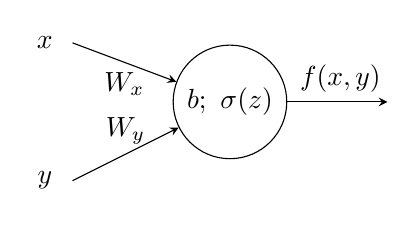
\begin{tikzpicture}
    		\tikzstyle{unit}=[draw,shape=circle,minimum size=1.15cm]
    		\node[unit](p) at (2,1){$b;\ \sigma(z)$};
		    \draw[->,>=stealth] (0,1.75) node[xshift=-10]{$x$} --(p) node[midway,below] {$W_x$};
    		\draw[->,>=stealth] (0,0) node[xshift=-10]{$y$} -- (p) node[midway,above] {$W_y$};
    		\draw[->,>=stealth] (p) -- (4,1) node[xshift=-17,above]{$f(x,y)$};
        \end{tikzpicture}
        \caption{Single perceptron model}
        \label{fig:simple_percep}
    \end{figure}
    We consider that each input has an associated weight \(W_x\) and \(W_y\), and that the node has an intrinsic bias \(b\) and an \textit{activation function} \(\sigma\). Given an input \(z = W_xx + W_yy + b\), the activation function determines the output of the node \(a = \sigma(z)\). This simple example can be thought of as a regression problem for the three parameters \(x\), \(y\) and the intercept \(b\). 
    % With this simple example we can think of the weights representing the coefficients for a linear regression problem of up to degree two and the bias as the intercept. 
    
    In the last \href{https://github.com/jgci2000/FYS-STK4155-projects/blob/master/project_1/doc/report_project1.pdf}{project}, we studied linear models that can perform a polynomial fit to a well-behaved function. We can then build upon the simple perceptron model. If we now let the one node have \(n\) inputs, we can solve a linear regression problem of degree \(n\), if we think of each input \(i\) as being \(x^i\), and each weight as being a coefficient in the linear expression. With this setup, we can also solve binary classification problems, by scaling the output and interpreting it as a probability.
    
    % Adding another node, we can now solve binary classification problems where, for example, if the first node activates we have a true output and if the second node activates the output is false. 
    
    Building further upon this model, by adding an additional layer between the input and output layer, we can create a so-called multi-layer perceptron model, Figure \ref{fig:multi_percep}. This we can solve even harder problems, e.g. image recognition and \(K\)-class classification problems. 
    \begin{figure}[htp]
        \centering
        \scalebox{0.75}{
            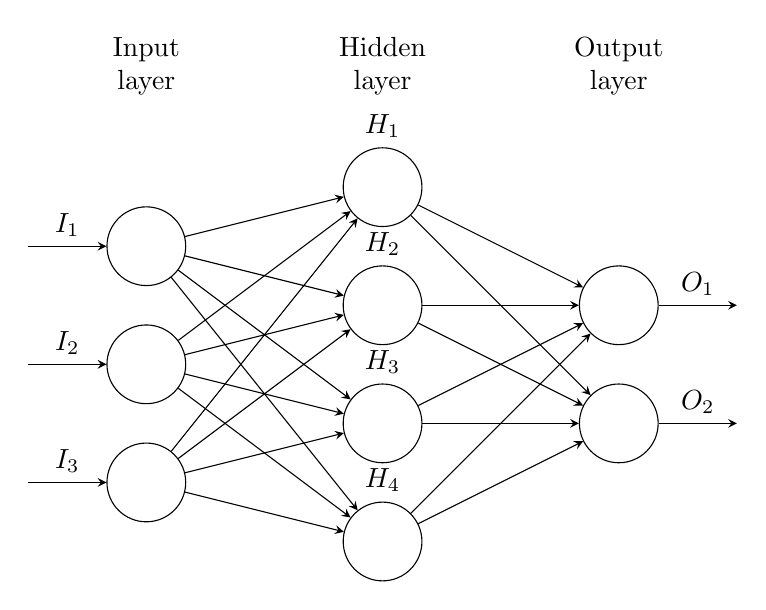
\begin{tikzpicture}[x=1.5cm, y=1.5cm, >=stealth]
            
            % Input nodes
            % \foreach \m/\l [count=\y] in {1,2,3,4}
            %   \node [every neuron/.try, neuron \m/.try] (input-\m) at (0,2.5-\y) {};
            \foreach \m/\l [count=\y] in {1,2,3}
              \node [every neuron/.try, neuron \m/.try] (input-\m) at (0,2-\y*1.) {};
              
            % Hidden nodes
            % \foreach \m [count=\y] in {1,missing,2}
            %   \node [every neuron/.try, neuron \m/.try ] (hidden-\m) at (2,2-\y*1.25) {};
            \foreach \m [count=\y] in {1,2,3,4}
              \node [every neuron/.try, neuron \m/.try ] (hidden-\m) at (2,2.5-\y) {};
                    
            % Output nodes
            % \foreach \m [count=\y] in {1,missing,2}
            %   \node [every neuron/.try, neuron \m/.try ] (output-\m) at (4,1.5-\y) {};
            \foreach \m [count=\y] in {1,2}
              \node [every neuron/.try, neuron \m/.try ] (output-\m) at (4,1.5-\y) {};
            
            % Input I with line
            % \foreach \l [count=\i] in {1,2,3,n}
            %   \draw [<-] (input-\i) -- ++(-1,0)
            %     node [above, midway] {$I_\l$};
            \foreach \l [count=\i] in {1,2,3}
              \draw [<-] (input-\i) -- ++(-1,0)
                node [above, midway] {$I_\l$};
            
            % Text above hidden nodes
            % \foreach \l [count=\i] in {1,n}
            %   \node [above] at (hidden-\i.north) {$H_\l$};
            \foreach \l [count=\i] in {1,2,3,4}
              \node [above] at (hidden-\i.north) {$H_\l$};
            
            % Text above output lines
            % \foreach \l [count=\i] in {1,n}
            %   \draw [->] (output-\i) -- ++(1,0)
            %     node [above, midway] {$O_\l$};
            \foreach \l [count=\i] in {1,2}
              \draw [->] (output-\i) -- ++(1,0)
                node [above, midway] {$O_\l$};
            
            % Lines from input nodes to hidden nodes
            % \foreach \i in {1,...,4}
            %   \foreach \j in {1,...,2}
            %     \draw [->] (input-\i) -- (hidden-\j);
            \foreach \i in {1,...,3}
              \foreach \j in {1,...,4}
                \draw [->] (input-\i) -- (hidden-\j);
            
            % Lines from hidden nodes to output nodes
            % \foreach \i in {1,...,2}
            %   \foreach \j in {1,...,2}
            %     \draw [->] (hidden-\i) -- (output-\j);
            \foreach \i in {1,...,4}
              \foreach \j in {1,...,2}
                \draw [->] (hidden-\i) -- (output-\j);
            
            % Position of text over layers
            \foreach \l [count=\x from 0] in {Input, Hidden, Output}
              \node [align=center, above] at (\x*2,2.2) {\l \\ layer};
            
            \end{tikzpicture}
        }
        \caption{Multi-layer perceptron model with one hidden layer.}
        \label{fig:multi_percep}
    \end{figure}
This model is known as a feedforward neural network. Such a network is assigned $L$ layers (layers 1 through \(L-1\) are the hidden layers, and layer \(L\) is the output layer), with \(n_{l}\) neurons (or nodes) in each layer. For each of the layers a weight matrix \(W^{(l)}\) of size \(n_{l} \times n_{l-1}\) is assigned, where the entry \(W^{(l)}_{ij}\) represents the weight that connects node \(i\) from layer \(l-1\) to node \(j\) into layer \(l\). Each layer is also assigned a bias vector \(b^{(l)}\) of size \(n_{l}\). To evaluate the networks predictions, we apply a cost function. This will determine the accuracy or error of our model. We wish to minimize this error. 

% A trained network has its weights and biases in all layers set to some combination of values that, together, ideally produce results in its output layer that are close to the desired target values for any valid input of size $n_{0}$. 

%The process by which we can use our model to make predictions is called feedforward.
We can use such a model to make predictions using the feed forward process.
The inputs can be denoted as $a^{(0)}$; then, for each layer, in turn, from $1$ to $L$, the layer's output $a^{(l)}$ (vector of size $n_{l}$) is computed as
\begin{align*}
    z^{(l)} &= W^{(l)} a^{(l-1)} + b^{(l)},
    \\
    a^{(l)} &= \sigma^{(l)} ( z^{(l)} ),
\end{align*}
where $\sigma^{(l)}$ is the layer's activation function. For a regression problem, the output layer's activation function should be the identity function, $\sigma^{(L)} : z_i \mapsto z_i$, as we wish to allow all values in \(\mathbb{R}\). On the other hand, for classification problems, as we desire a probabilistic output, the prediction should be contained in \([0, 1]\). This way, we can use a sigmoid function,
\begin{equation*}
    \sigma^{(L)}(z_i) = \frac{1}{1+e^{-z_i}},
\end{equation*}
or any other function of the type \(\mathbb{R} \to [0, 1]\). A usual example is the softmax
\begin{equation*}
    \sigma^{(L)}(z_i) = \frac{e^{z_i}}{\sum_{j = 1}^{n_l} e^{z_j}}
\end{equation*}
or the hyperbolic tangent
\begin{equation*}
    \sigma^{(L)}(z_i) = \tanh (z_i).
\end{equation*}

Additionally, we explore using different activation functions in the hidden layers, amongst the sigmoid, the hyperbolic tangent, the rectified linear unit (ReLU) function
\begin{align*}
    \sigma^{(l)}(z_i) = 
    \begin{cases}
        z_i &z_i \geq 0
        \\
        0 &z_i < 0,
    \end{cases}
\end{align*}
the leaky ReLu
\begin{align*}
    \sigma^{(l)}(z_i) = 
    \begin{cases}
        z_i &z_i \geq 0
        \\
        \alpha z_i &z_i < 0,
    \end{cases}
\end{align*}
and the exponential linear unit (ELU) function
\begin{align*}
    \sigma^{(l)}(z_i) = 
    \begin{cases}
        z_i &z_i \geq 0
        \\
        \alpha \left(e^{z_i} - 1\right) &z_i < 0,
    \end{cases}
\end{align*}
with \(0 < \alpha \ll 1\).

% It is common courtesy to initialize out weights and biases randomly.
Typically, the weights and biases in the network are initialized randomly, corresponding to an initial guess.
It is then highly unlikely to produce good predictions. In order to obtain accurate prediction with our network, the weights and biases are iteratively adjusted until the predictions given by the network are satisfactory. This process is called \textit{training}. In this process we use gradient methods to find the minimum of the model's cost function. We are now faced with a problem of computing the gradients of the cost function with respect to all of the weights and biases that comprise the network. As the network has potentially hundreds of weights and biases all dependant on each other, this becomes quite computationally heavy to do naively. Luckily, there is an algorithm that can efficiently compute the task at hand: \textit{backpropagation}. A short overview is presented here; for an in-depth derivation of the expressions shown, see \hyperref[sec:backprop]{Appendix B}.

Depending on the way we initialize the weights and biases, we might get a faster convergence or non-convergence of the employed gradient method. We initialize the biases to some small value $\epsilon$ (the value of which we can experiment with to find the best initial value), and the weights with uniform distribution between $-1$ and $1$. %Then, over a number of epochs, the training data, or, depending on the method employed, smaller batches taken out of the full set, is repeatedly fed forward through the network. Each time, the output error is computed as the gradient of the cost function times the derivative of the output layer's activation function.

The way we update the weights and biases each epoch is given by
\begin{align*}
    W^{(l)} &\xleftarrow{} W^{(l)} - \eta \frac{\partial C}{\partial W^{(l)}}
    \\
    b^{(l)} &\xleftarrow{} b^{(l)} - \eta \frac{\partial C}{\partial b^{(l)}}.
\end{align*}
To compute the gradients of the cost function with respect to the weights and biases, we used the backpropagation algorithm, which consists of computing
\begin{align*}
    \frac{\partial C}{\partial z^{(L)}} &= \frac{\partial C}{\partial a^{(L)}}\odot\sigma^{L\prime}(z^{(L)}),
    \\
    \frac{\partial C}{\partial z^{(l)}} &= \sigma^{(l)\;\prime}(z^{(l)})\odot((W^{(l+1)})^T\delta^{(l+1)}),
    \\
    \frac{\partial C}{\partial b^{(l)}} &= \delta^{(l)},
    \\
    \frac{\partial C}{\partial W^{(l)}} &= \delta^{(l)}(a^{(l-1)})^T,
\end{align*}
where \(\delta^{(l)} := \frac{\partial C}{\partial z^{(l)}}\).

Once all weights and biases throughout the network have been updated epoch times, the hope is that our cost function decreases.

Additionally, to prevent overfitting, we can introduce a regularization term in the cost function \cite{hastie}. For an \(\ell_2\) regularization term the updated gradients will take the form
\begin{align*}
    W^{(l)} &\xleftarrow{} W^{(l)} - \eta \left( \frac{\partial C}{\partial W^{(l)}} + \lambda W^{(l)} \right)
    \\
    b^{(l)} &\xleftarrow{} b^{(l)} - \eta \left( \frac{\partial C}{\partial b^{(l)}} + \lambda b^{(l)} \right),
\end{align*}
where \(\lambda\) is a hyperparameter for the regularization term, and \(C\) is the cost function without regularization.

%%%%%%%%%%%%%%%%%%%%%%%%%%%
%%%%%%%%%%%%%%%%%%%%%%%%%%%
\section*{Implementation}
%%%%%%%%%%%%%%%%%%%%%%%%%%%
%%%%%%%%%%%%%%%%%%%%%%%%%%%

The core neural network implementation is written in an object-oriented, component-based manner. As reference previously, the code can be found on \href{https://github.com/jgci2000/FYS-STK4155-projects/tree/master/}{GitHub}. The central \texttt{Neural\-Network.\linebreak[0]Model.\linebreak[0]Model} class represents the full network, to be trained and run on a number of different continuous and classification problems.

The base \texttt{Neural\-Network.\linebreak[0]Layer.\linebreak[0]Layer} abstract class, inherited by \texttt{Neural\-Network.\linebreak[0]Layer.\linebreak[0]Hidden\-Layer} and \texttt{Neural\-Network.\linebreak[0]Layer.\linebreak[0]Output\-Layer} for syntax clarity, represents a single layer with \(n\) neurons, instances of which can be added as components to a \texttt{Model} instance.

When adding new layers to a \texttt{Model} instance, in order of forward execution (i.e. with the output layer at the end), the size of each layer is needed (as \texttt{Layer::\linebreak[0]\_size}), as well as the size of the previous layer (determined automatically from the model's input size for the first layer, or from the last stacked layer's size), and one of the \texttt{Neural\-Network.\linebreak[0]Activation\-Functions} sibling classes as the activation function, which provides the function itself and its first derivative.

The available activation functions for hidden layers are the sigmoid, hyperbolic tangent, ELU, ReLU and leaky ReLU. Regarding our softmax function implementation, one thing to note is that the \(\sum_{j = 1}^{n_l} e^{z_j}\) term is very quick to explode to very large numbers, yielding \texttt{NaN}s in the output as a result - instead, we compute softmax as \(e^S\), with
\begin{align*}
    S &= \ln\left(e^{z_i}\right) - \ln\left(\sum_{j = 1}^{n_l}e^{z_j}\right)
    \\
    &= z_i - \left(\ln\left(\sum_{j = 1}^{n_l}e^{z_j}\right) - \ln\left(e^7\right)\right) - 7
    \\
    &= z_i - 7 - \ln\left(\sum_{j = 1}^{n_l}\frac{e^{z_j}}{e^7}\right)
\end{align*}
Since \(e^7 \approx 1100\) is a much larger number than individual \(e^{z_i}\) terms expected from normalized data points, this expression turns out much more stable computationally.

The feedforward step is done by the \texttt{Model::\linebreak[0]feed\_\linebreak[0]forward} method, to which the inputs are passed as a matrix of size $k\times s$, where $s$ = \texttt{Model::\linebreak[0]\_input\_\linebreak[0]size}, and $k$ any number of data points; the output is given as a $k\times n^{(L)}$ matrix, where $n^{(L)}$ is the size of the output layer. This output is obtained by internally repeatedly calling the \texttt{Layer::\linebreak[0]forward} method on each layer sequentially, which computes the layer's output as
\begin{align*}
    z^{(l)} &= W^{(l)} a^{(l-1)} + b^{(l)}
    \\
    a^{(l)} &= \sigma ( z^{(l)} )
\end{align*}
These results are obtained fully via NumPy matrix operations (including the activation function execution), in order to speed up execution.

Training the network, either via \texttt{Model::\linebreak[0]train}, to train the model once over a number of epochs with a given learning rate and hyperparameters, using either GD or SGD, or via \texttt{Model::\linebreak[0]grid\_\linebreak[0]train} in order to vary any 2 parameters and train the network repeatedly to find the best fit, internally relies on the \texttt{Model::\linebreak[0]back\_\linebreak[0]prop} method, itself calling \texttt{Layer::\linebreak[0]backward} on each layer in reverse order, which computes the weight and bias gradients, updating the individual neurons by
\begin{align*}
    W^{(l)} &\xleftarrow{} W^{(l)} - \eta (a^{(l-1)} \delta^{(l)} + \lambda W^{(l)} )
    \\
    b^{(l)} &\xleftarrow{} b^{(l)} - \eta (\delta^{(l)\;T} + \lambda b^{(l)} )
\end{align*}
Where \(z^{(l)}\) is the non-activated output of layer \(l\) as a vector of size \(n_{l}\), \(a^{(l)} = \sigma^{(l)} (z^{(l)} )\), \(\eta\) the learning rate and \(\lambda\) the regularization parameter; the column vector error \(\delta^{(l)}\) is given by
\begin{align*}
    \delta_l = 
    \begin{cases}
        C^{\,\prime} (a^{(L)\;T} ) \odot \sigma^{L\;\prime} (z^{(L)\;T} ) &l = L
        \\
         (\delta^{(l+1)} W^{(l+1)} ) \odot \sigma^{(l)\;\prime} (z^{(l)\;T} ) &l \neq L
    \end{cases}
\end{align*}

The convenience method \texttt{Model::\linebreak[0]error} feeds forward once with the given inputs and returns \(C (a^{(L)} )\); i.e. the MSE of the output for regression problems, and the accuracy of the output for classification problems.

%%%%%%%%%%%%%%%%%%%%%%%%%%%
%%%%%%%%%%%%%%%%%%%%%%%%%%%
\section*{Discussion}
%%%%%%%%%%%%%%%%%%%%%%%%%%%
%%%%%%%%%%%%%%%%%%%%%%%%%%%

%%%%%%%%%%%%%%%%%%%%%%%%%%%
\subsection*{Regression on Franke's Function}
%%%%%%%%%%%%%%%%%%%%%%%%%%%
% Part a,b,c

In order to test the implementation of the optimization methods discussed above, we start by running our linear regression models on Franke's function \cite{franke1979critical}. The data we feed to our models is 1000 uniformly scattered points on \([0,1]\times[0,1]\), sampled as
\begin{equation*}
    z = F(x, y) + \epsilon
\end{equation*}
where \(F: \mathbb{R}^2 \xrightarrow{} \mathbb{R}\) is Franke's function and \(\epsilon\sim N\left(0, \sigma \right)\) follows a normally distributed noise, with \(\sigma=\frac{1}{4}\) throughout.

\begin{table}[htp]
    \centering
    \caption{Time, in milliseconds, per epoch for SGD and GD for different learning rate values, averaged over 100 separate runs of 200 epochs each to reduce statistical noise. The size of each batch was set to \(5\). Computation time taken from system with an i7 4790 @ 3.60 GHz.}
    \begin{tabular}[t]{c|c c|c c}
        Method & \multicolumn{2}{c|}{SGD (200 batches)} & \multicolumn{2}{c}{GD} \\
        \hline & & & & \\
        \(\eta\) & 0.01 & 0.001 & 0.01 & 0.001 \\
        \hline & & & & \\
        Time per epoch (ms) & \(1.69\) & \(1.00\) & \(0.17\) & \(0.13\) \\
        & & & & \\
        Time per step (ms) & \(8.5\cdot10^{-3}\) & \(5.0\cdot10^{-3}\) & 0.17 & 0.13
    \end{tabular}
    \label{tab:time_epoch}
\end{table}
\begin{figure}[htp]
    \centering
    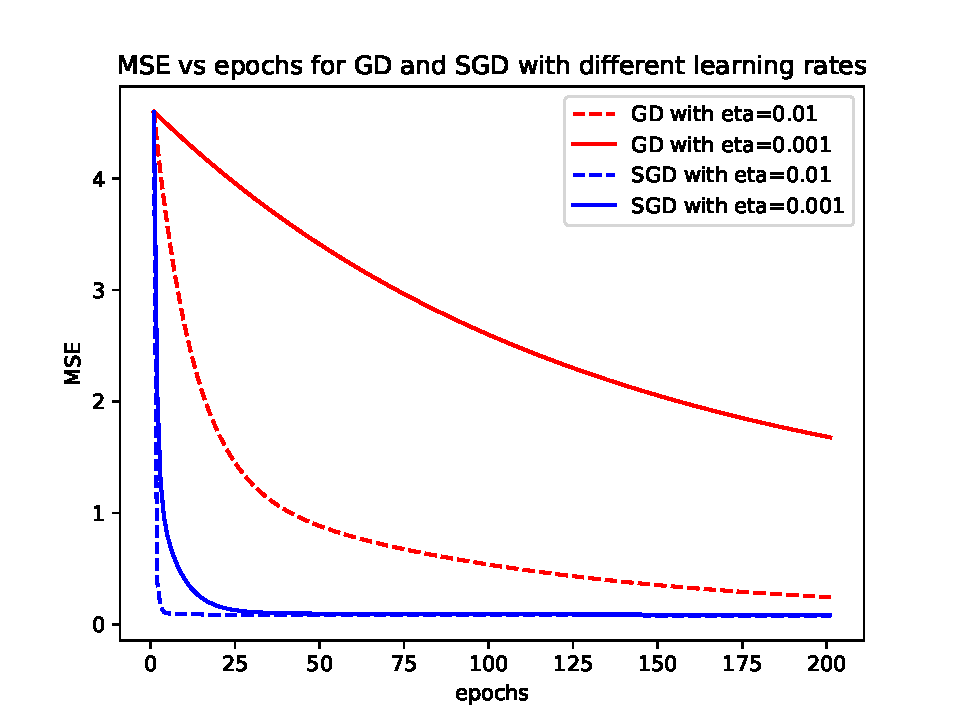
\includegraphics[width=\linewidth]{part_a/1_mse_eta_epochs_200_s_bathes_5.pdf}
    \caption{MSE for Franke's function as a function of epochs for Gradient Descent and Stochastic Gradient Descent methods for two different values of the learning rate \(\eta\). The batch size for SGD is 5.}
    \label{fig:mse_epochs_gd_sgd}
\end{figure}
\begin{figure}[htp]
    \centering
    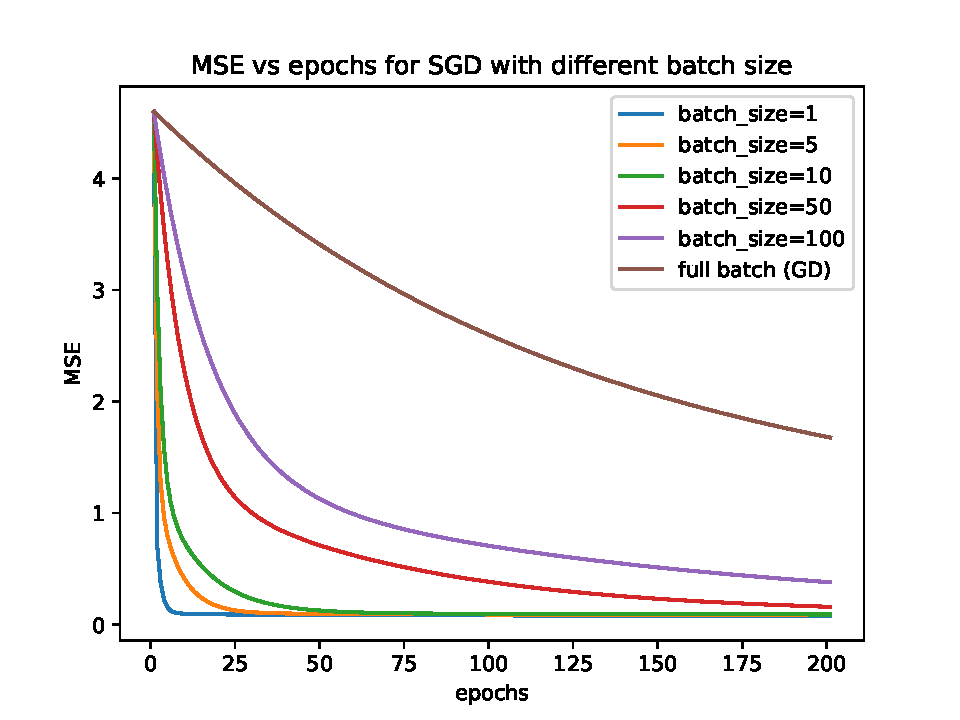
\includegraphics[width=\linewidth]{part_a/2_mse_batch_size_epochs_200_eta_0.001.pdf}
    \caption{MSE for Franke's function as a function of epochs for SGD optimizer as a function of the batch size. The learning rate is \(0.001\). As the batch size increases, the MSE over epochs behaves like GD's MSE.}
    \label{fig:mse_epochs_bat_size}
\end{figure}

In Figure \ref{fig:mse_epochs_gd_sgd} we can find the comparison between the error of SGD and GD over epochs for two different learning rates. We see that SGD converges faster for both learning rates than GD. Furthermore, in Figure \ref{fig:mse_epochs_bat_size}, we can see that as we increase the batch size, the convergence rate of SGD approaches the convergence rate of GD.

Since \(\lfloor \frac{N}{M} \rfloor = \frac{1000}{5} = 200\) steps are performed in each epoch of the SGD method while only one is done with GD, it is expected for SGD to take longer per epoch than GD. Indeed, each SGD epoch takes around 9 times longer to compute compared to GD, Table \ref{tab:time_epoch}. That being said, the time per individual step with SGD is much lower than with GD since gradients are computed from 5 points at a time instead of 1000. Thus, SGD and GD achieve very similar MSEs after the same amount of steps, but SGD does so in a much faster fashion in terms of real time taken. Furthermore, due to the random nature of SGD, there is a possibility for encountered local minima to be overcome since there is no confinement to a predetermined path on the n-dimensional MSE surface. Knowing this, we can conclude that SGD is a more efficient and reliable method.
%\\[6pt]
% A comparison of the convergence rates of GD and SGD with different values of the learning rate \(\eta\) gives a predictable result; a higher learning rate produces a higher convergence rate to the minimum MSE found with both methods, Figure \ref{fig:mse_epochs_gd_sgd}. Note that with a value of \(\eta\) too large (e.g. \(\eta=1\)), the computation overflows in the first few epochs.

\begin{figure}[htp]
    \centering
    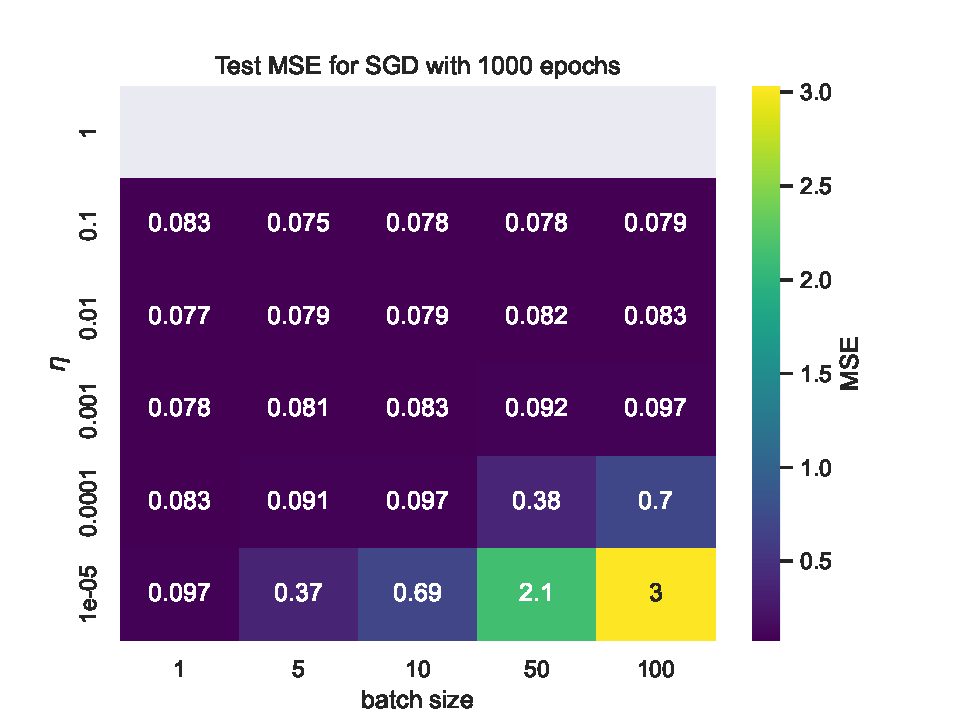
\includegraphics[width=\linewidth]{part_a/3_mse_eta_size_batch_epochs_1000.pdf}
    \caption{Grid search for the optimal MSE for Franke's function as a function of the batch size and learning rate \(\eta\). The number of epochs used is \(1000\). The grey squares indicate that the method was not able to converge due to numerical overflow.}
    \label{fig:grid_mse_batch_eta}
\end{figure}

In Figure \ref{fig:grid_mse_batch_eta}, we have plotted a grid search for the optimal MSE over different learning rates and batch sizes for the SGD method. Through the analysis of the figure, we can see that for learning rates lower that \(10^{-4}\), the MSE worsens, since the limited number of epochs did not enable the method to converge. Again showing that as the number of batches decreases, the convergence rate also decreases. Thus, for a fast and accurate convergence, we restrict ourselves to a batch size of 5 and learning rates higher than \(10^{-4}\). For large learning rates, the method is not able to converge due to numerical overflow.

% Comparing the resulting MSE obtained via SGD with varying learning rates and mini-batch sizes after a set number of epochs, Figure \ref{fig:grid_mse_batch_eta}, we find the ideal combination to be using batches of size \(5\) (for \(1000\) data points, this corresponds to \(200\) mini-batches), and \(\eta\approx0.1\). Note that while this may indicate the highest possible learning rate should always be chosen to converge as quickly as possible, a learning rate that is too high (e.g. \(\eta=1\)) ends up producing an undefined MSE (and undefined outputs) as a result of a large divergence. As discussed above, the theoretical maximum \(\eta\) is the inverse of the largest of the eigenvalues of the hessian matrix, but since the hessian isn't known in the general case, the optimal learning rate needs to be searched for and approximated depending on the problem at hand to be as large as possible within the range of acceptable values.

\begin{figure}[h!]
    \centering
    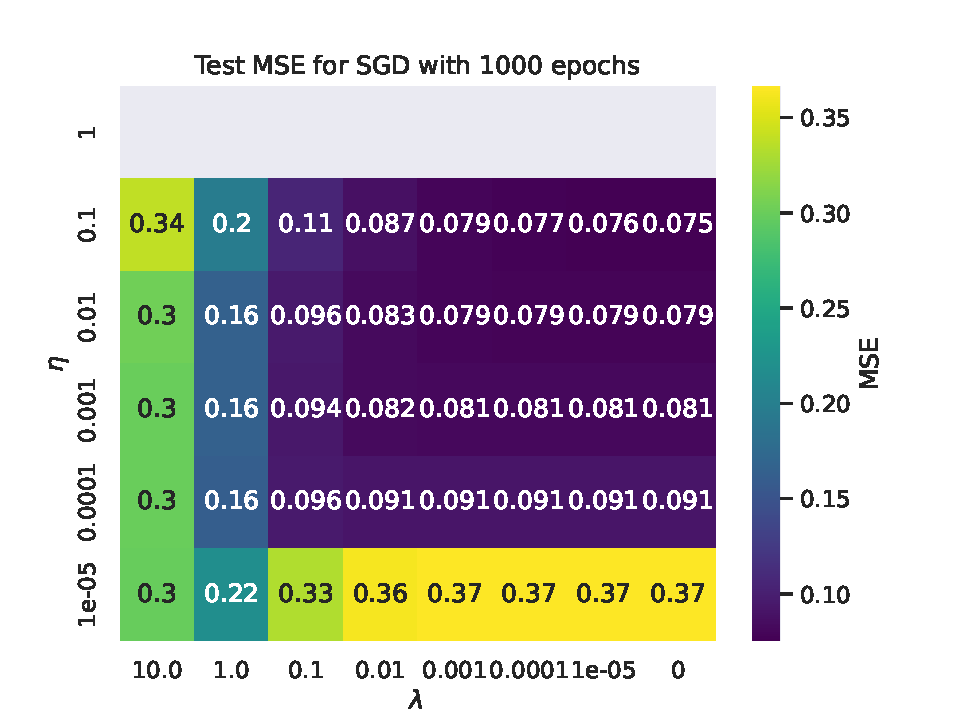
\includegraphics[width=\linewidth]{part_a/4_mse_eta_reg_epochs_1000.pdf}
    \caption{Grid search for the optimal MSE for Franke's function as a function of the learning rate \(\eta\) and \(\ell_2\) regularization parameter \(\lambda\). The number of epochs used is \(1000\). The grey squares indicate that the method was not able to converge due to numerical overflow. This shows that the combination of batch size and learning rate is not optimal for these values - here in particular, \(\eta = 1\) is too high of a learning rate.}
    \label{fig:grid_mse_lmd_eta}
\end{figure}

Introducing \(\ell_2\) regularization and keeping the optimal mini-batch size found above, we can compare results produced by different combinations of parameters \(\eta\) and \(\lambda\), as shown in Figure \ref{fig:grid_mse_lmd_eta}. In this particular case, \(\ell_2\) regularization is found to produce worse results than the original \(\lambda=0\) samples, and the best MSE is still found at \((\eta,\lambda)=(0.1,0)\) after 1000 epochs. This result is to be expected, since we have already shown the polynomial fit to Franke's function to be better modeled by ordinary least squares than ridge regression.

We have also tested how an adaptive learning rate affects our models ability to fit Franke's function. We have found no benefits of using an adaptive scheme for the learning rate. Furthermore finding the optimal values for \(t_0\) and \(t_1\) might pose to be a tedious and unrewarding process, as the convergence rate does not change significantly.

\begin{figure}[h!]
    \centering
    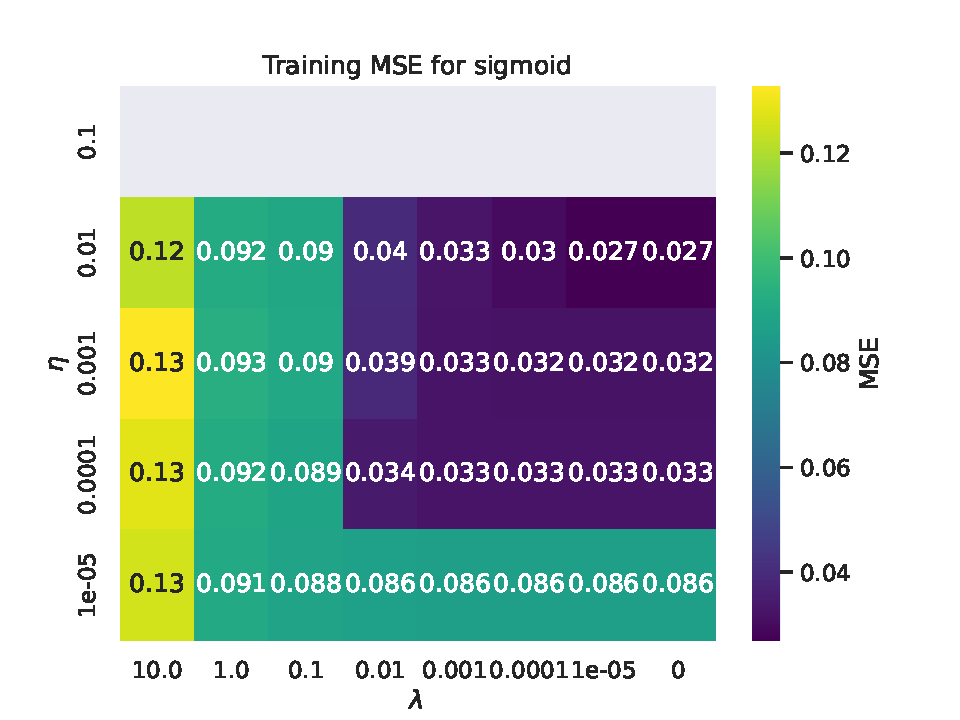
\includegraphics[width=\linewidth]{figures/part_b/1_grid_search_sigmoid.pdf}
    \caption{Grid search for the optimal MSE for Franke's function with our feedforward neural network as a function of the learning rate \(\eta\) and \(\ell_2\) regularization parameter \(\lambda\). The network is composed of one hidden layer with 30 nodes and a sigmoid as an activation function. The number of epochs used is \(1000\). The grey squares indicate that the method was not able to converge due to numerical overflow.
    %This shows that the combination of regularization parameter and learning rate is not optimal.
    }
    \label{fig:nn_grid_mse_lmd_eta_sigmoid}
\end{figure}

In order to solve the same regression problem with our feedforward neural network implementation, we initialize a network with a single hidden layer with 30 neurons, with a sigmoid as the activation function. The input layer is of size \(2\), and the output layer is of size \(1\), with a linear activation function, in order to fit points \(f(x, y) = F(x, y) + \epsilon\) as \(a^{(L)} \overset{!}{=} f (a^{(0)}_0, a^{(0)}_1 )\). The network is trained via SGD, with again a batch size of 5.

Performing the same analysis as we did for OLS and Ridge with SGD, we have produced a grid search over various values of the learning rate and regularization parameter, Figure \ref{fig:nn_grid_mse_lmd_eta_sigmoid}. We have found again, that a low regularization parameter produces the best results to fit Franke's function, with a learning rate higher than \(10^{-4}\). However, the MSE is about 2 times lower than with OLS and Ridge solved by SGD. We again observe that high learning rates cause numerical overflow.

% With a sigmoid as the activation function used for the hidden layer, we find the best combination of \((\eta,\lambda)\) after 1000 epochs to be \((\eta,\lambda)\approx(10^{-2},10^{-3})\), Figure \ref{fig:nn_grid_mse_lmd_eta_sigmoid}. In this particular case, low values of the regularization parameter combined with any valid learning rate gives MSEs in the same ballpark, a possible indication that such a neural network is quicker to converge to the final MSE than the regression methods for different values of \(\eta\) and \(\lambda\).

\begin{figure}[htp]
    \centering
    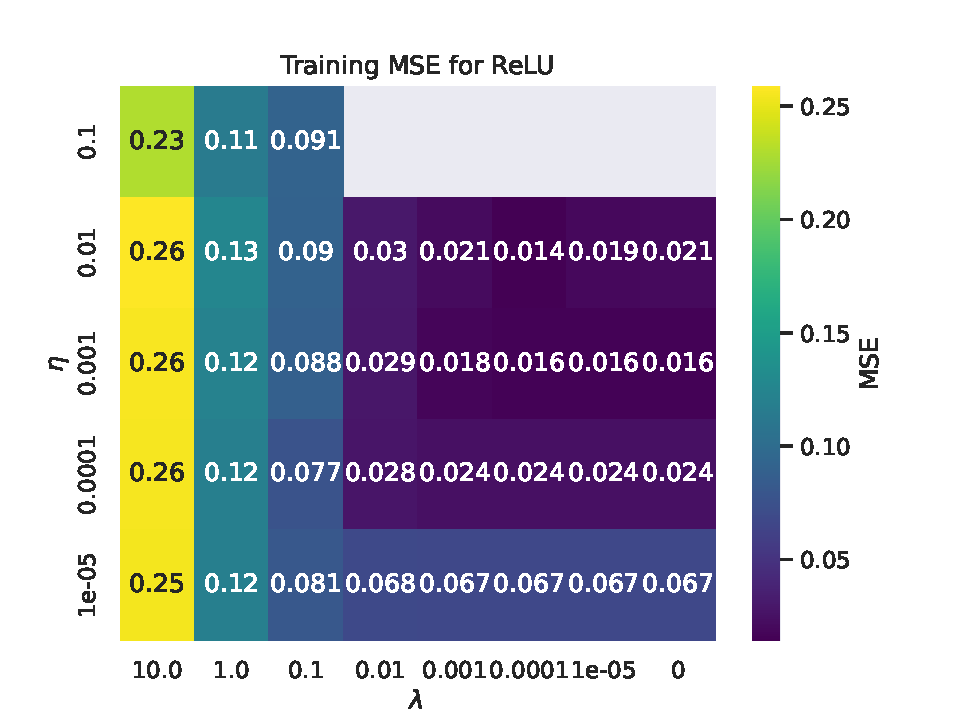
\includegraphics[width=\linewidth]{figures/part_b/2_grid_search_relu.pdf}
    \caption{Grid search for the optimal MSE for Franke's function with our feedforward neural network as a function of the learning rate \(\eta\) and \(\ell_2\) regularization parameter \(\lambda\). The network is composed of one hidden layer with 30 nodes and a ReLU as an activation function. The number of epochs used is \(1000\). The grey squares indicate that the method was not able to converge due to numerical overflow.}
    \label{fig:nn_grid_mse_lmd_eta_relu}
\end{figure}

For a similar network with the activation function of the hidden layer set to a ReLU, we observe better results than with the sigmoid, especially with \(\eta=10^{-3}\) and \(\lambda\leq10^{-4}\), Figure \ref{fig:nn_grid_mse_lmd_eta_relu}.

Comparing the MSE obtained after a fixed number of epochs, varying the number of hidden layers, we observe a much lower MSE for 9 or less layers than for more; in particular, the best fits arise as a result of 2 to 6 20-node hidden layers in this case after 500 epochs, Figure \ref{fig:mse_hidd_lay}. This shows that increasing the model complexity does not mean automatically that get a lower error. This should be kept in mind when studying more complex problems.

Building a network with two hidden layers (both using the sigmoid as the activation function), we compare differences in predictions given by initializing the neurons' biases to either 0 or 1, Figure \ref{fig:mse_init_bias}. The predictions over the first few epochs are much closer for a lower initial bias, but the two variants produce results very close to each other after a dozen iterations, although in the long run, the MSE for networks initialized with a higher bias tends to be ever so slightly lower than with a lower initial bias (in this case, \(\text{MSE}_{\text{initial bias} = 1} \approx 0.135\) and \(\text{MSE}_{\text{initial bias} = 0} \approx 0.140\)).

\begin{figure}[htp]
    \centering
    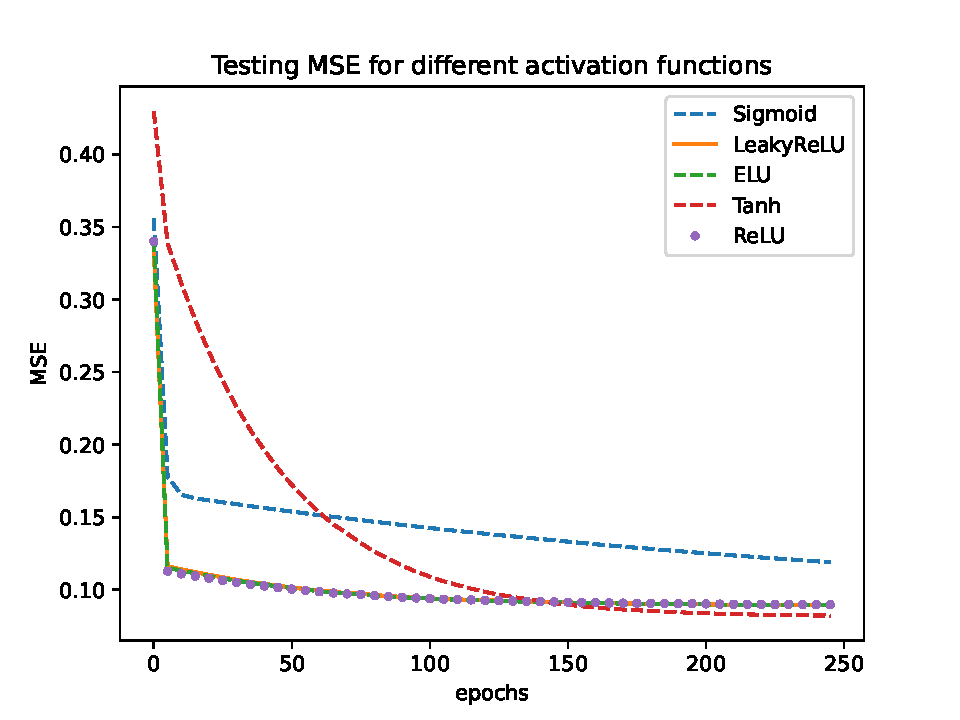
\includegraphics[width=\linewidth]{part_c/1_mse_epochs_activ_funcs.pdf}
    \caption{MSE for Franke's function with our feedforward neural network as a function of epochs for different activation functions. Here, the ELU and Leaky ReLU are both computed with \(\alpha=0.05\). The network is composed of a 2 hidden layers with 20 nodes each and an output layer.  The first hidden layer has a sigmoid as an activation function and the second hidden layer can have different activation functions. The output layer as a linear function as the activation function.}
    \label{fig:mse_activ_func}
\end{figure}

From Figure \ref{fig:mse_activ_func}, generally speaking, for the case of predicting Franke's function, the sigmoid, leaky ReLU, ReLU and ELU all converge at equivalent rates, with the sigmoid producing worse fits; using the hyperbolic tangent as the activation function results in a network that takes more time to converge, but results in a lower MSE. It's interesting to note that the ReLU, leaky ReLU and ELU produce largely identical results to each other (which incidentally makes this a difficult plot to show) over the same number of epochs in this particular setup.

%%%%%%%%%%%%%%%%%%%%%%%%%%%
\subsection*{Classification on the MNIST Data Set}
%%%%%%%%%%%%%%%%%%%%%%%%%%%
% Part d,e with MNist

In the last section, we have shown that out implementation of SGD and of a feedforward neural network is correct for linear regression type problems. In this section our aim is to validate its capabilities of classifying data correctly. For this we decided to use a subset of the MNIST data set, provided by SciKit Learn \cite{mnistsklearn}. This data set contains about 1800 labeled 8 by 8 pixels images of handwritten digits form 0 to 10, Figure \ref{fig:mnist_data_set}.

% The neural network therefore produces expected results for the linear regression problem with Franke's function as the data set; before we can apply the same model to the breast cancer data set, we test its classification capabilities on the MNIST handwritten digit samples database subset included in the SciKit Learn distribution, \cite{mnistsklearn}.

\begin{figure}[h]
    \centering
    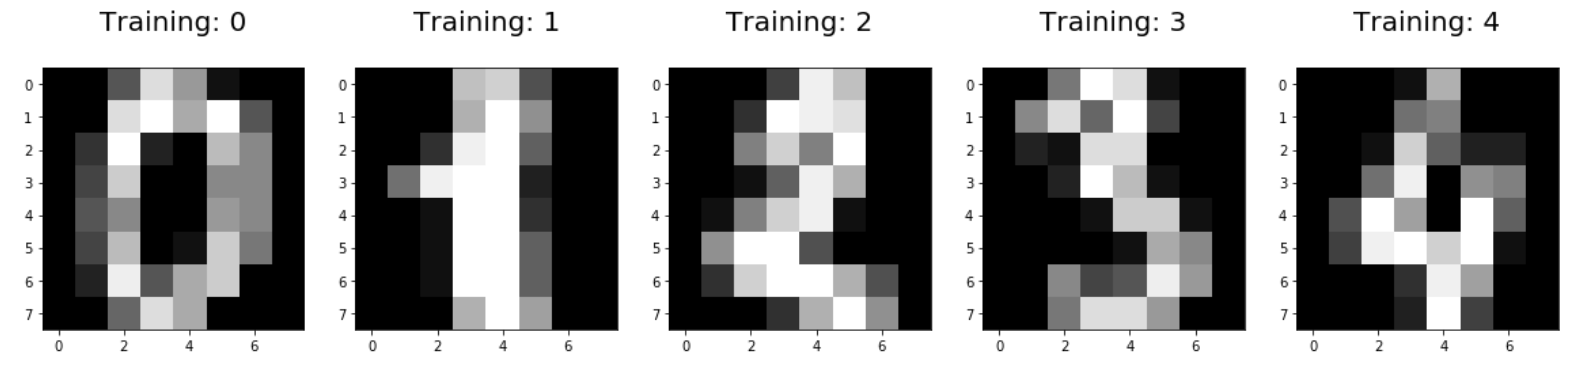
\includegraphics[width=\linewidth]{a.png}
    \caption{Example of data points from the MNIST data set.}
    \label{fig:mnist_data_set}
\end{figure}

To analyse this data set, we tested different neural networks architectures and found that the one that produced better results was a neural network with two hidden layers, with 20 nodes each and a sigmoid as the activation function. The output layer also uses a sigmoid as the activation function, but with 10 output nodes. We also used SGD as the gradient method, with a batch size of 5, over 500 epochs. 

\begin{figure}[htp]
    \centering
    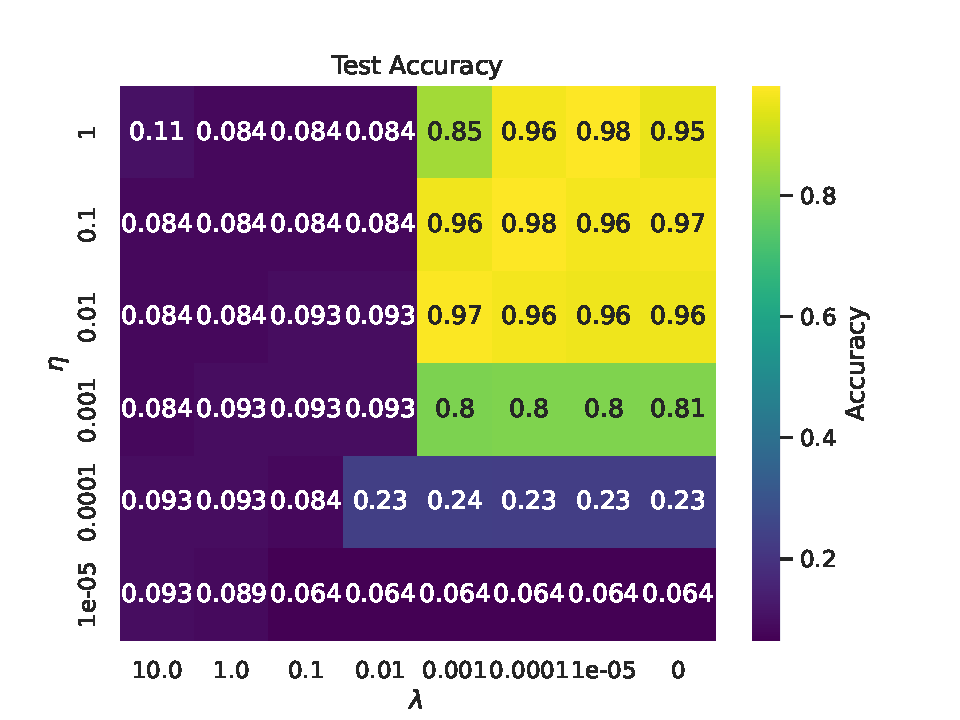
\includegraphics[width=\linewidth]{part_d/1_grid_search_mnist.pdf}
    \caption{Grid search for the optimal MSE for the MNIST dataset with our feedforward neural network as a function of the learning rate and regularization parameter. The number of epochs was }
    \label{fig:gs_mnist}
\end{figure}

In Figure \ref{fig:gs_mnist}, we can observe the grid search for accuracy of our network on the classification of the MNIST data set, for different values of the learning rate and regularization parameter. We found that, instead of a lower learning rate, this classification problem performs better with a higher learning rate value. 

A noteworthy aspect is that out neural network can successfully classify at best \(98\%\) the test data points.

%%%%%%%%%%%%%%%%%%%%%%%%%%%
\subsection*{Classification on the Wisconsin Breast Cancer Data Set}
%%%%%%%%%%%%%%%%%%%%%%%%%%%
% Part d,e with cancer

Having tested our implementation of a feedforward neural network on Franke's function and the MNIST data set, we now move on to the study of the famous Wisconsin Breast Cancer data set. This data set is comprised of features, such as area, radius, texture, etc, taken from medical imaging, of potentially tumours, labeled as malignant or benign.

In Figure \ref{fig:cov_cancer}, we can see the correlation matrix for the Breast Cancer data set. As it is expected, we find a high correlation between features such as mean radius and mean area or mean perimeter. To note, mean radius, mean area and mean perimeter all share a high correlation with mean concave points.

\begin{figure}[htp]
    \centering
    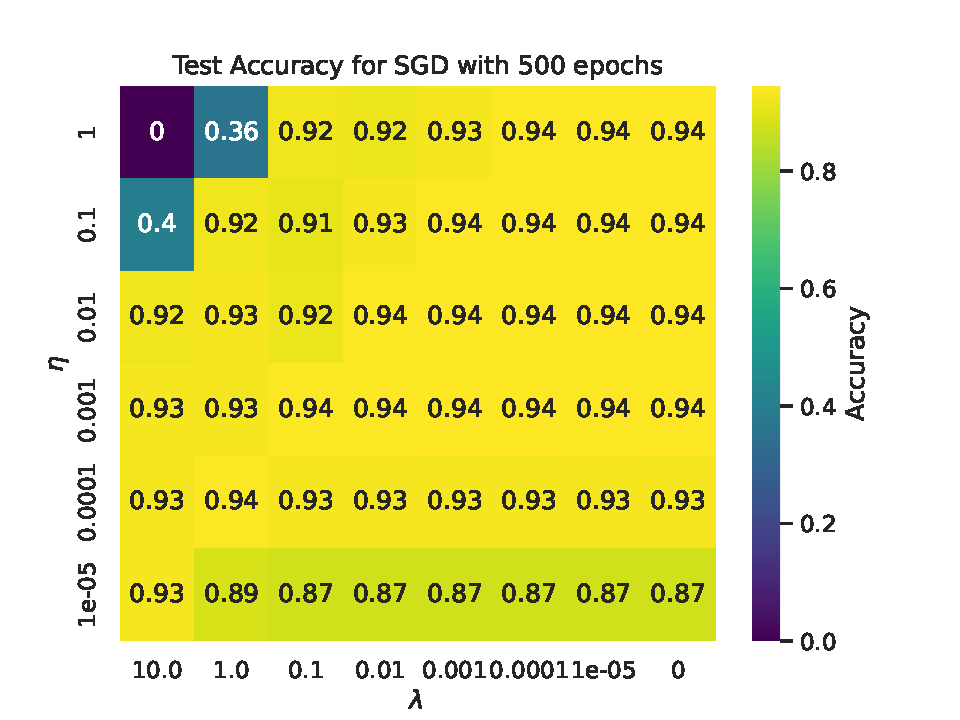
\includegraphics[width=\linewidth]{part_e/1_cancer_log_reg_500_epochs.pdf}
    \caption{Grid search for the optimal MSE for the cancer data with standard logistic regression as a function of the learning rate \(\eta\) and \(\ell_2\) regularization parameter \(\lambda\) using SGD. The number of epochs used is \(500\).}
    \label{fig:gs_log_reg_cancer}
\end{figure}

We first use standard logistic regression, where we initialize the features vector with a uniform distribution between 0 an 1, with SGD as the gradient method. In Figure \ref{fig:gs_log_reg_cancer}, we see a grid search for the optimal values of the learning rate and regularization parameter. After 500 epochs, we find an accuracy of \(94\%\) at best with various hyperparameter combinations, especially at lower values of the regularization parameter \(\lambda \leq 0.01\) and higher values of the learning rate \(\eta \geq 10^{-3}\).

We repeat the same exercise with our feedforward neural network. We tested a vast array of architectures and found good results with a network with 2 hidden layers, each with 20 nodes and the sigmoid as the activation function. The output layer also uses a sigmoid as the activation function. We also used the cross-entropy as the cost function, since we are dealing with a classification problem.

\begin{figure}[htp]
    \centering
    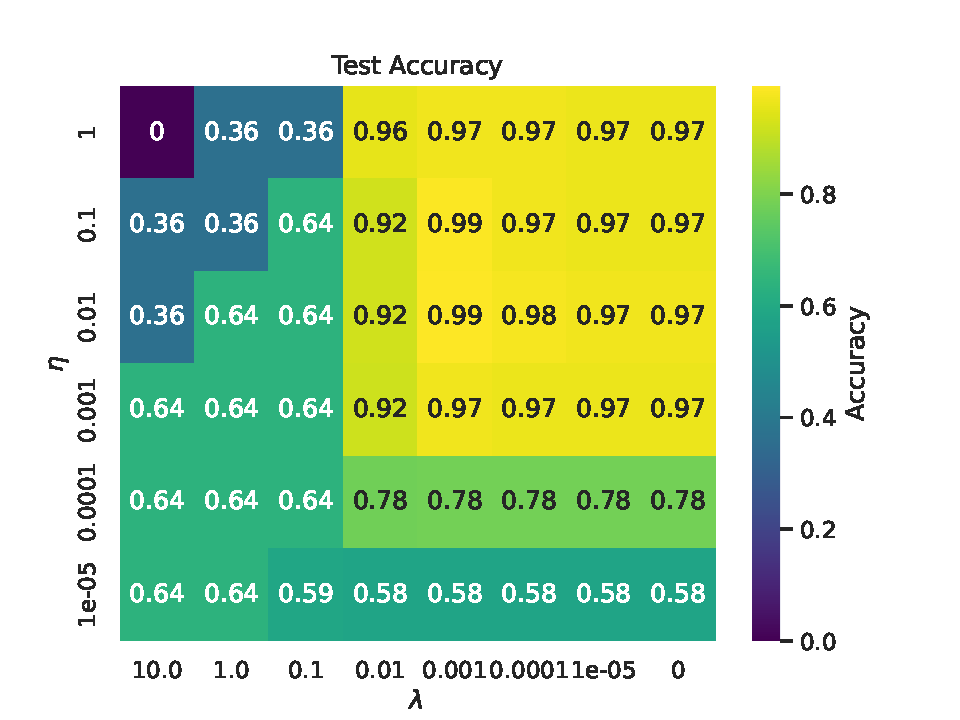
\includegraphics[width=\linewidth]{part_d/2_grid_search_cancer.pdf}
    \caption{Grid search for the optimal MSE for the cancer data with our feedforward neural network as a function of the learning rate \(\eta\) and \(\ell_2\) regularization parameter \(\lambda\) using SGD. The number of epochs used is \(500\).}
    \label{fig:gs_nn_cancer}
\end{figure}

In Figure \ref{fig:gs_nn_cancer}, we can see that the accuracy of the predictions, compared with logistic regression, increases to around 99\%, after 500 epochs, for \(\eta \in \left[0.1, 0.01\right]\), \(\lambda = 10^{-3}\). However, the accuracy decreases faster as a function of the distance to the optimal learning rate and regularization parameter than with standard logistic regression: with \((\eta,\lambda)=(10^{-5},1)\), we obtain \(\text{Accuracy}_{\text{SGD}}\approx0.89\) whereas \(\text{Accuracy}_{\text{FFNN}}\approx0.64\). This is an indication that, while the neural network has the potential to perform better, it is more sensitive to the hyperparameters, meaning there's a higher guarantee to obtain better predictions with standard linear regression from a naive starting set of \((\eta,\lambda)\) without the added overhead brought by the tweaking of these parameters.

We noted while testing out some architectures on our neural network, some of which we were expecting to fail, such as having no hidden layers and a linear function as the output layer's activation function, that the network could surprisingly reproduce 95\% of the test Breast Cancer data set correctly. However, in this case, we cannot interpret the output of the neural network as probabilities anymore, since some are negative or larger than 1. This shows that even though the test accuracy might seem high, the interpretation might be wrong, so it is in the user's interest to always double-check the validity of the network.
% We noted while testing out some architectures of neural networks, we tried some that were expect to fail. Such as having no hidden layers and a linear function as the outputs layer activation function. We tested this with the Breast Cancer data set, and, surprisingly, found out that we were able to reproduce \(95\%\) of the test set correctly. However, in this case, we can not interpret the output of the neural network as probabilities, as some are negative or larger than 1. This shows that even though the test accuracy might seem high, the interpretation might be wrong, so it is by the users interest to always double check the validity of the network. 

%%%%%%%%%%%%%%%%%%%%%%%%%%%
%%%%%%%%%%%%%%%%%%%%%%%%%%%
\section*{Conclusion}
%%%%%%%%%%%%%%%%%%%%%%%%%%%
%%%%%%%%%%%%%%%%%%%%%%%%%%%
% Part f

We started by studying and comparing the performance of gradient methods, namely Gradient Descent and mini-batch Stochastic Gradient Descent. We found that mini-batch Stochastic Gradient Descent is more efficient and reliable than Gradient Descent given that the number of batches is relatively small and it can overcome confinement to local minima.

We implemented a code for a feedforward neural network  with a flexible number of layers, nodes per layer and a vast array of activation functions to choose from. The training process is achieved by optimization methods, using the backpropagation algorithm for fast computation of gradients. This network was tested for both regression and classification problems to validate its performance. We also found that Rectified Linear Unit, leaky Rectified Linear Unit and Exponential Linear Unit as cost functions can provide a faster convergence of the mean squared error, while the hyperbolic tangent might give slower convergence.

Firstly, we applied both the neural network and standard linear regression models with mini-batch Stochastic Gradient Descent to data generated by Franke's function. We found that the linear model (\(\text{MSE} \approx 0.075\)) performs slightly worse than our neural network (\(\text{MSE} \approx 0.027\)).

We then applied this functioning network code to a subset of the MNIST data set and found that out network is able to achieve an accuracy of \(98\%\) on the recognition of low-resolution handwritten digits.

Lastly, we studied the Wisconsin Breast Cancer data set, and found some expected and some unexpected correlations between some of the features of the data set. We also applied standard logistic regression with mini-batch Stochastic Gradient Descent and a neural network to compare their performance. We found that logistic regression might give a worse accuracy (\(94\%\)) than with the neural network (\(99\%\)), although it is less susceptible to changes in hyperparameters.

We have shown that our feedforward neural network implementation is a suitable adaptive model to predict both regression- and classification-type problems. In particular, this machine learning implementation predicts better results than standard regression models for the Wisconsin Breast Cancer data set, our focus data.


\bibliography{refs.bib}


\appendix
\section{Figures}

% \subsection{Linear Regression}
% LINEAR REGRESSION SECTION
% \begin{figure}[htp]
%     \centering
%     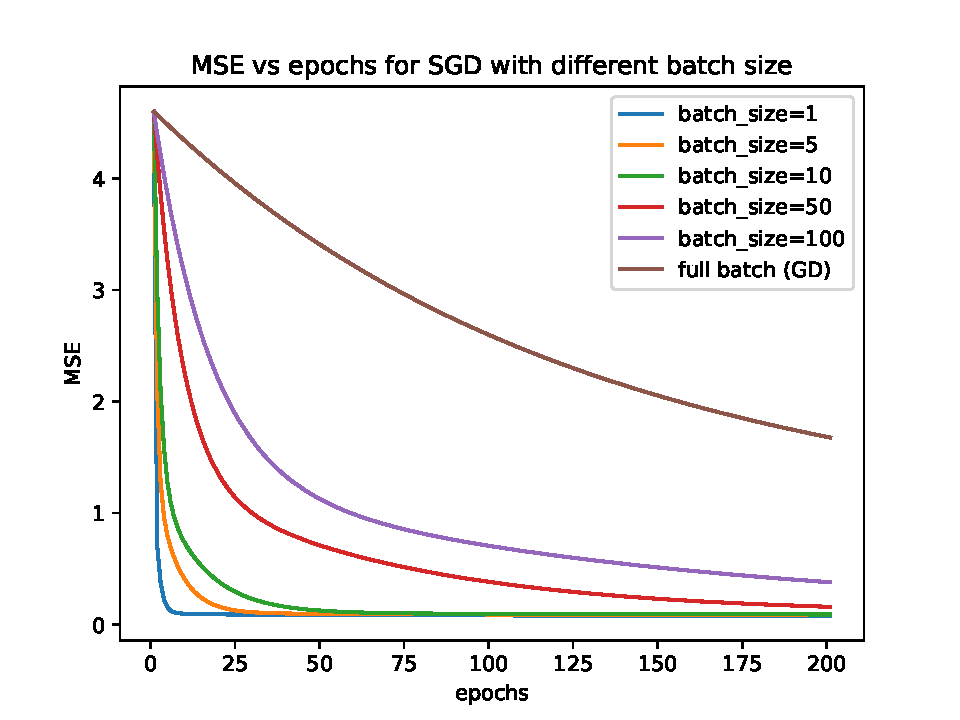
\includegraphics[width=\linewidth]{part_a/2_mse_batch_size_epochs_200_eta_0.001.pdf}
%     \caption{MSE as a function of epochs for SGD optimizer as a function of the batch size. The learning rate is \(0.001\). As the batch size increases, the MSE over epochs behaves like GD's MSE.}
%     \label{fig:mse_epochs_bat_size}
% \end{figure}

% \begin{figure}[htp]
%     \centering
%     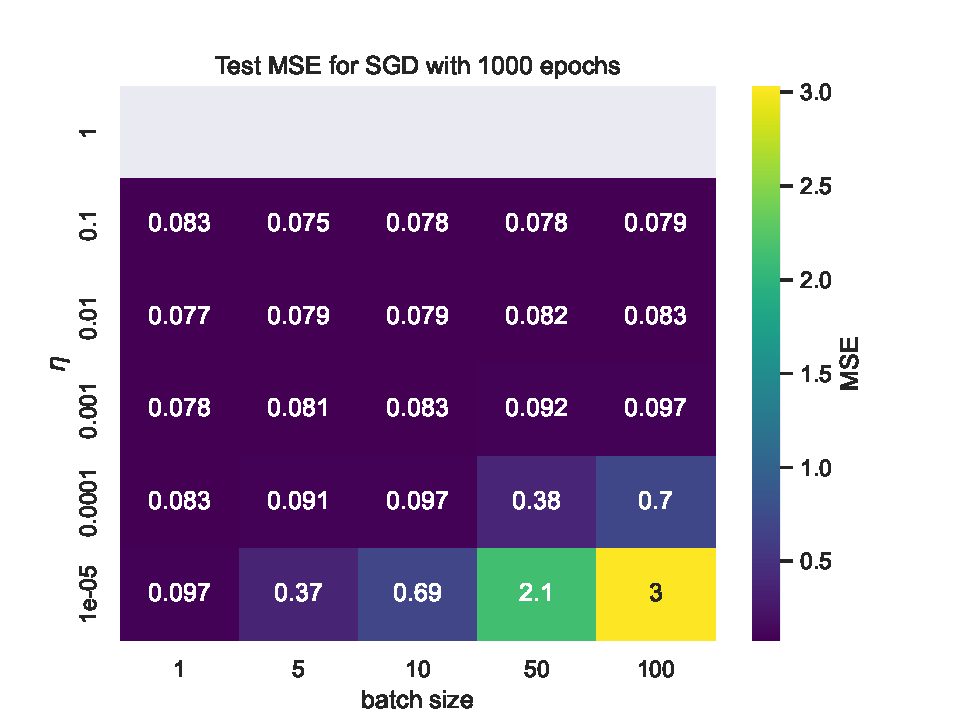
\includegraphics[width=\linewidth]{part_a/3_mse_eta_size_batch_epochs_1000.pdf}
%     \caption{Grid search for the optimal MSE as a function of the batch size and learning rate \(\eta\). The number of epochs used is \(1000\). The grey squares indicate that the method was not able to converge due to numerical overflow.}
%     \label{fig:grid_mse_batch_eta}
% \end{figure}



% \begin{figure}[htp]
%     \centering
%     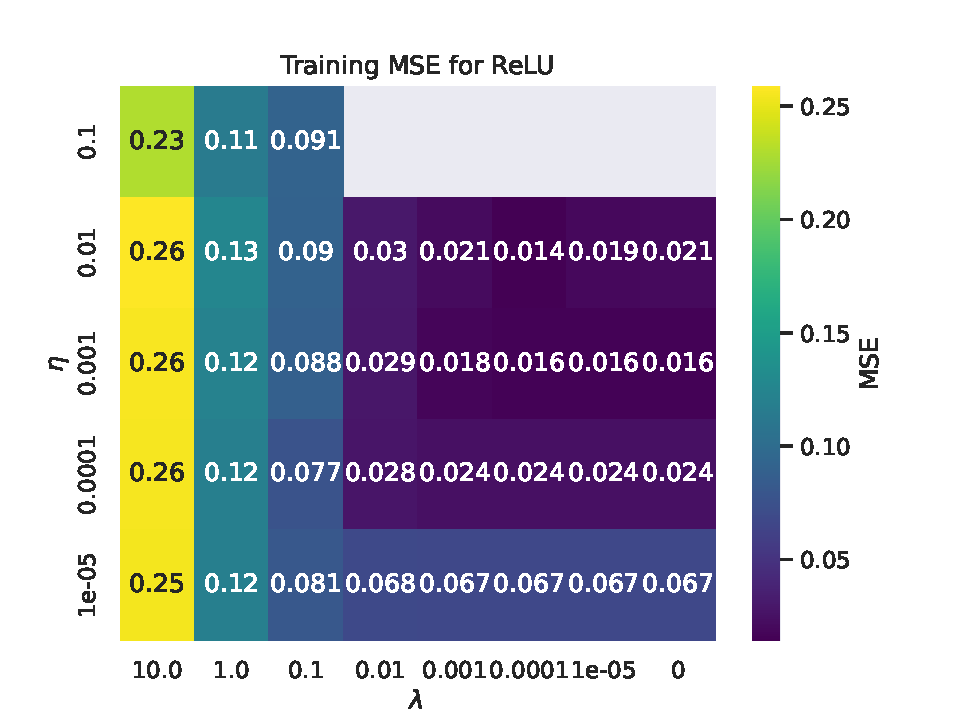
\includegraphics[width=\linewidth]{figures/part_b/2_grid_search_relu.pdf}
%     \caption{Grid search for the optimal MSE as a function of the learning rate \(\eta\) and \(\ell_2\) regularization parameter \(\lambda\). The network is composed of one hidden layer with 30 nodes and a ReLU as an activation function. The number of epochs used is \(1000\). The grey squares indicate that the method was not able to converge due to numerical overflow.}
%     \label{fig:nn_grid_mse_lmd_eta_relu}
% \end{figure}

\begin{figure}[htp]
    \centering
    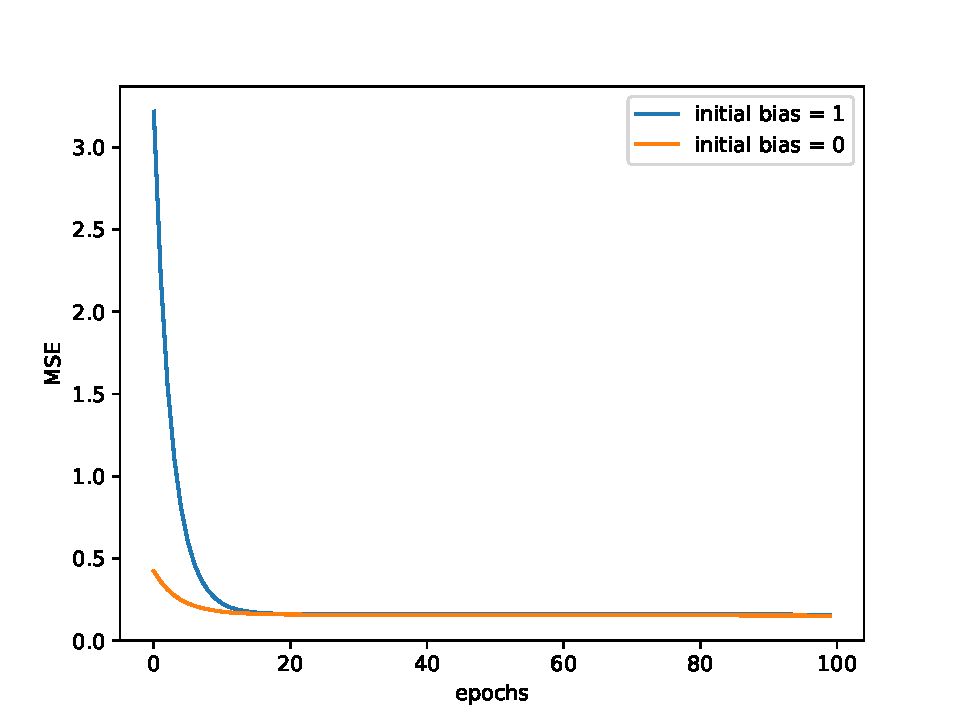
\includegraphics[width=\linewidth]{part_c/2_init_bias_comp.pdf}
    \caption{MSE for Franke's function with our feedforward neural network as a function of epochs for two different ways of initializing the bias vector. The network is composed of a 2 hidden layers with 20 nodes each and a sigmoid as the activation function, and an output layer.}
    \label{fig:mse_init_bias}
\end{figure}

\begin{figure}[htp]
    \centering
    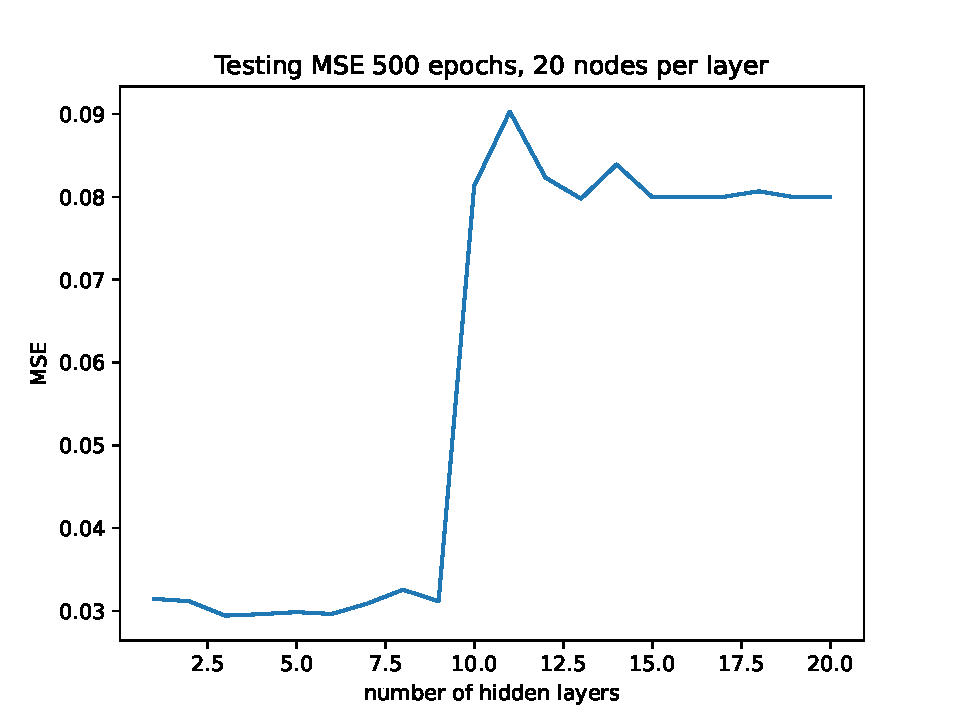
\includegraphics[width=\linewidth]{figures/part_c/3_mse_layers.pdf}
    \caption{MSE for Franke's function with our feedforward neural network as a function of hidden layers after 500 epochs. Each hidden layer has 20 nodes, with the sigmoid as the activation function.}
    \label{fig:mse_hidd_lay}
\end{figure}

% LOGISTIC REGRESSION

% \subsection{Cancer Data}
% CANCER

% \begin{figure}[htp]
%     \centering
%     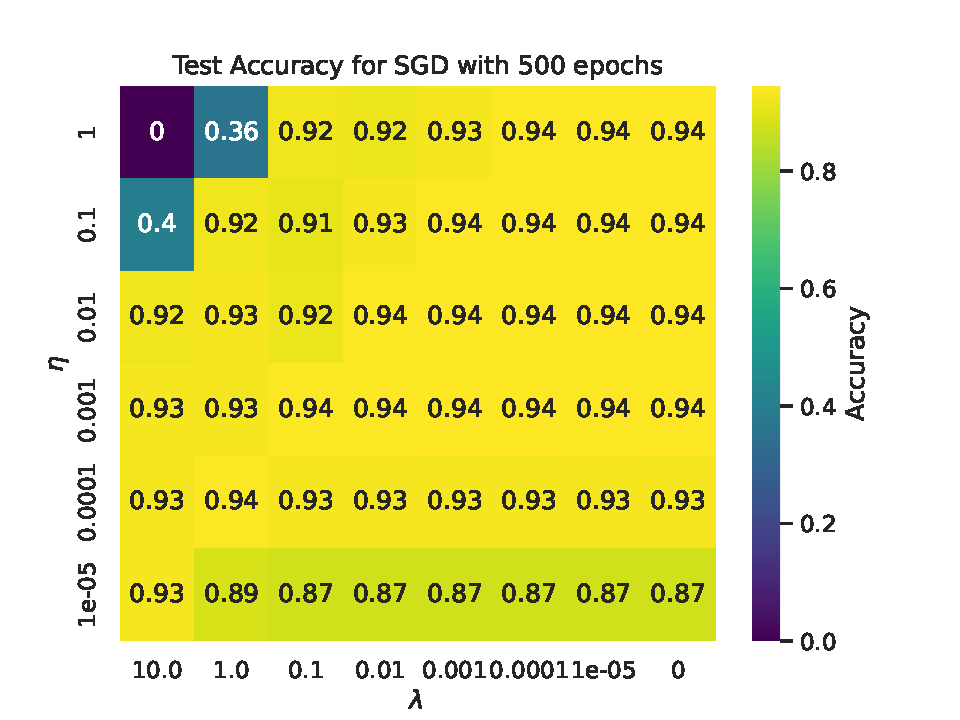
\includegraphics[width=\linewidth]{part_e/1_cancer_log_reg_500_epochs.pdf}
%     \caption{Grid search for the optimal MSE as a function of the learning rate \(\eta\) and \(\ell_2\) regularization parameter \(\lambda\). The number of epochs used is \(500\).}
%     \label{fig:gs_log_reg_cancer}
% \end{figure}

% \begin{figure}[htp]
%     \centering
%     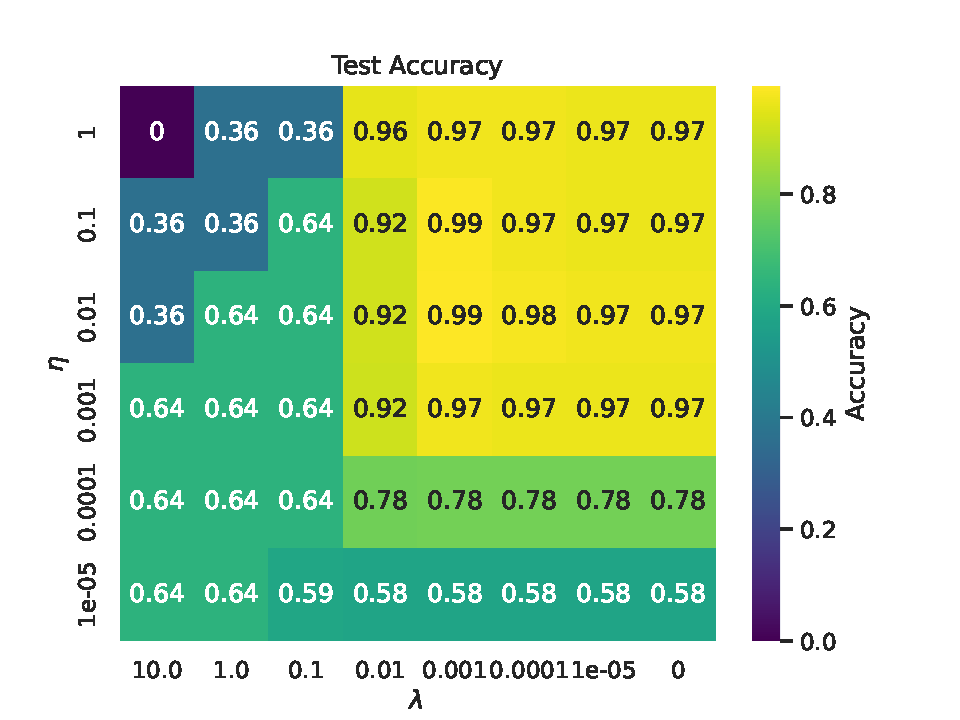
\includegraphics[width=\linewidth]{part_d/2_grid_search_cancer.pdf}
%     \caption{Grid search for the optimal MSE as a function of the learning rate \(\eta\) and \(\ell_2\) regularization parameter \(\lambda\). The number of epochs used is \(500\).}
%     \label{fig:gs_nn_cancer}
% \end{figure}

\clearpage

\onecolumngrid
\begin{figure*}[htp]
    \centering
    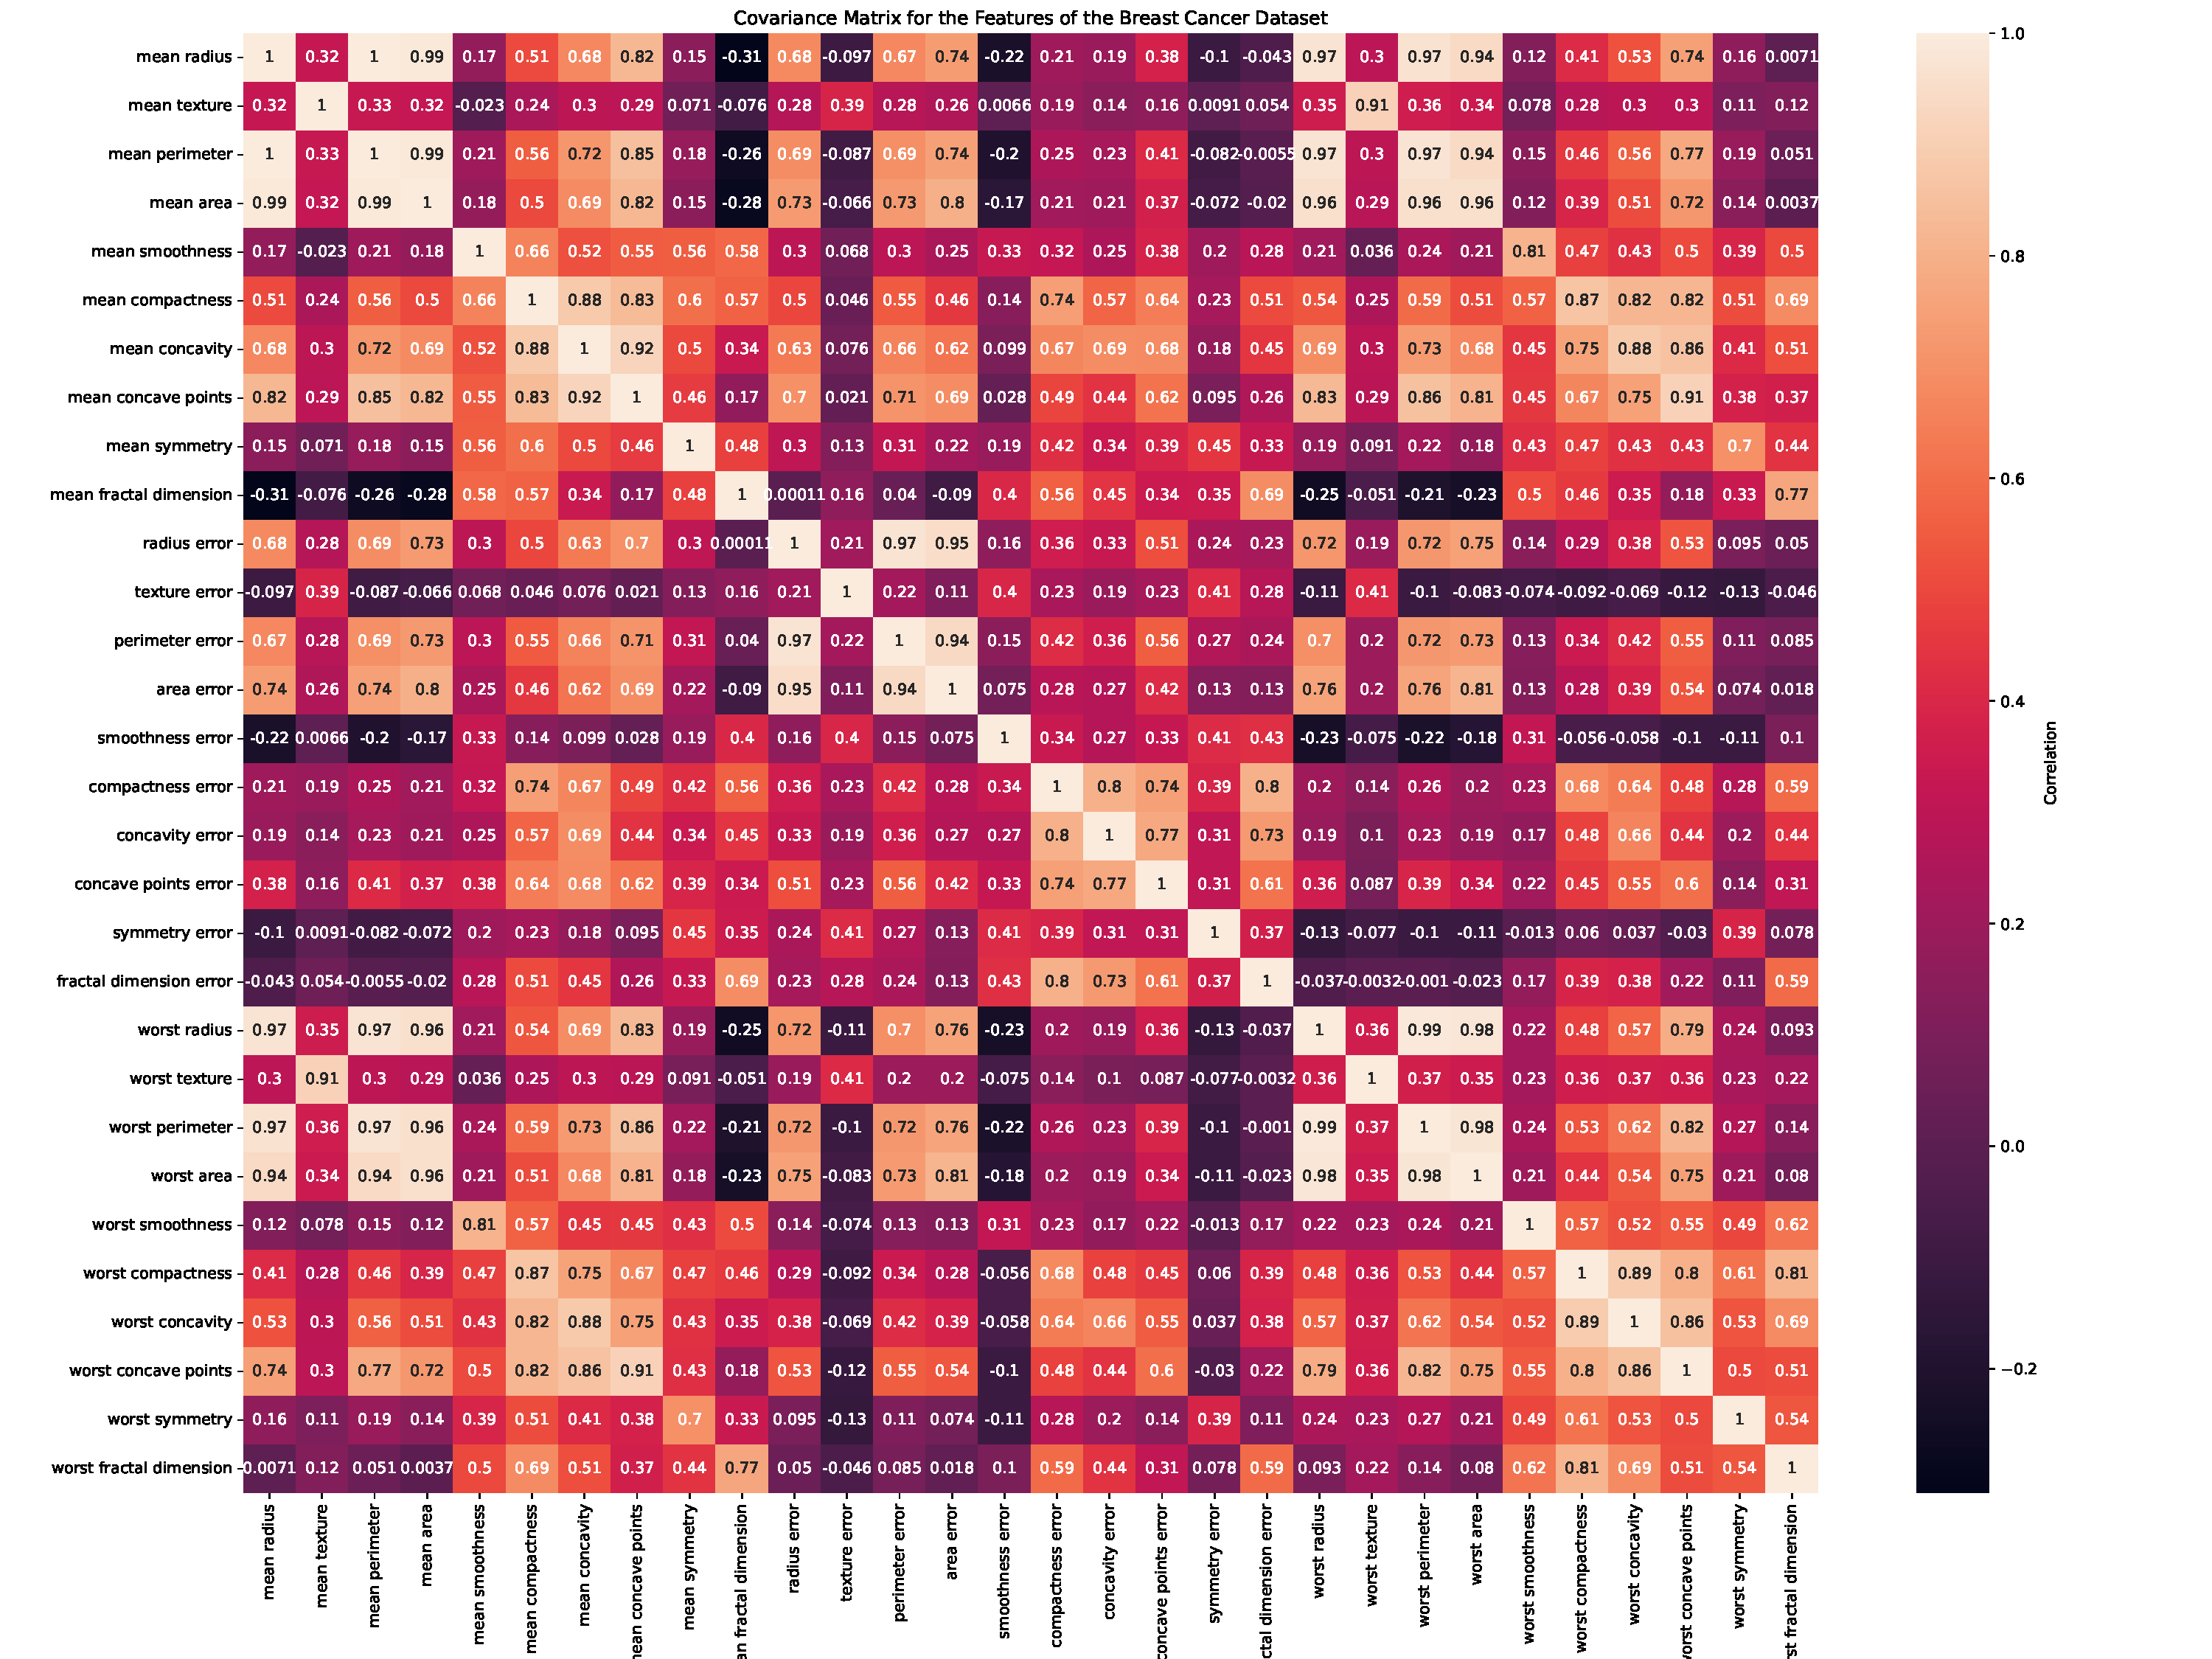
\includegraphics[scale=0.325]{corr_cancer.pdf}
    \caption{Correlation matrix for the features of the Wisconsin Brest Cancer data set.}
    \label{fig:cov_cancer}
\end{figure*}

\clearpage

\section{Backpropagation}
\label{sec:backprop}

Define \(z^{(l)}=W^{(l})a^{(l-1)}+b^{(l)}\), i.e. the weighted sum of the activation of the previous layer, and \(a^{(l)}=\sigma^{(l)}(z^{(l)})\), where \(\sigma^{(l)}\) is the activation function of layer \(l\). Assume further that the cost fucntion can be written as
\begin{align*}
    &C(a^{(L)}_1(x_1),\ldots,a^{(L)}_1(x_n),a^{(L)}_2(x_1),\ldots,a^{(L)}_2(x_n),\ldots,a^{(L)}_{n_L}(x_n))=\sum_{i=1}^n\sum_{k_L}^{n_L}C_{i,k_L}(a^{(L)}_{k_L}(x_i)),
\end{align*}
where \(a^{(L)}_{k_L}(x_i)\) is the output of the activation of node \(a^{(L)}_{k_L}\) with respect to the datapoint \(x_i\), and \(C_{i,n_L}\) is the cost function using only the output \(a^{(L)}_{k_L}\). Denoting \(\delta^{(l)}_j:=\frac{\partial C}{\partial z^{(l)}_j}\), backpropagation consist of computing
\begin{align}
    \frac{\partial C}{\partial z^{(L)}_j} &= \frac{\partial C}{\partial a^{(L)}_j}\sigma^{(L)\;\prime}(z^{(L)}_i), \label{eq:backprop1}
    \\
    \frac{\partial C}{\partial z^{(l)}_j} &= \sigma^{(l)\;\prime}(z^{(l)}_j)\cdot\sum_{i=1}^{n_l}W^{(l+1)}_{ij}\delta^{(l+1)}_i, \label{eq:backprop2}
    \\
    \frac{\partial C}{\partial b^{(l)}_j} &= \delta^{(l)}_j, \label{eq:backprop3}
    \\
    \frac{\partial C}{\partial W^{(l)}_{jk}} &= a^{(l-1)}_k\delta^{(l)}_j. \label{eq:backprop4}
\end{align}
We derive these equations for a single data point. It is from this easy to generalize to the full cost function. Let \(n_l\) denote the number of nodes in layer \(l\), \(\sigma^{(l)}\) be the activation function of layer \(l\), \(a^{(l)}_i\) be the activation \(\sigma^{(l)}(z^{(l)}_i)\) of node \(i\) in layer \(l\) (for \(l=0\) the activation will be the input), \(z^{(l)}_i=\sum_{j=1}^{n_l}W_{ij}^{(l)}a^{(l-1)}_j+b^{(l)}_i\) be the weighted sum of the inputs to node \(i\) in layer \(l\). We let \(z^{(l)}=(z^{(l)}_1,\ldots,z^{(l)}_{n_l})^T\), where \(\sigma^{(l)}(z^{(l)})=(\sigma^{(l)}(z^{(l)}_1),\ldots,\sigma^{(l)}(z^{(l)}_{n_l}))^T\), and \(a^{(l)}=(a^{(l)}_1,\ldots,a^{(l)}_{n_l})^T\). Denote the final layer by \(L\). Notice that we can write the cost function as \(C(a^{(L)})=\sum_{k_L=1}^{n_L}C_{k_L}(a^{(L)}_{k_L})\). We begin by computing
\begin{align*}
    \frac{\partial C}{\partial z^{(L)}_i}=\sum_{k_L=1}^{n_L}\frac{\partial}{\partial z^{(L)}_i}C_{k_L}(a^{(L)}_{k_L})=\sum_{k_L=1}^{n_L}\frac{\partial C_{k_L}}{\partial a^{(L)}_{k_L}}\frac{\partial a^{(L)}_{k_L}}{\partial z^{(L)}_i}&=\frac{\partial C_i}{\partial a^{(L)}_i}\sigma^{(L)\;\prime}(z^{(L)}_i)
    \\
    &=\sigma^{(L)\;\prime}(z^{(L)}_i)\sum_{k_L=1}^{n_L}\frac{\partial C_{k_L}}{\partial a^{(L)}_i}=\frac{\partial C}{\partial a^{(L)}_i}\sigma^{(L)\;\prime}(z^{(L)}_i):=\delta^{(L)}_i
\end{align*}
In general we will have
\begin{equation*}
    \frac{\partial z^{(l)}_i}{\partial z^{(l-1)}_j}
    =\frac{\partial}{\partial z^{(l-1)}_j}\left(\sum_{k_{l-1}}^{n_{l-1}}W_{ik_{l-1}}^{(l)}\sigma^{(l-1)}(z^{(l-1)}_{k_{l-1}})+b^{(l)}_i\right)
    =W_{ij}^{(l)}\sigma^{(l-1)\;\prime}(z^{(l-1)}_j).
\end{equation*}
To see how we get to the general case, we look at how we can compute \(\delta^{(L-1)}_i\) and \(\delta^{(L-2)}_i\). We get
\begin{align*}
    \frac{\partial C}{\partial z^{(L-1)}_i}
    &=\sum_{k_L=1}^{n_L}\frac{\partial C_{k_L}(\sigma^{(L)}(z^{(L)}_{k_L}))}{\partial z^{(L-1)}_i}
    =\sum_{k_L=1}^{n_L}\frac{\partial C_{k_L}(\sigma^{(L)}(z^{(L)}_{k_L}))}{\partial z^{(L)}_{k_L}}\frac{\partial z^{(L)}_{k_L}}{\partial z^{(L-1)}_i}
    =\sum_{k_L=1}^{n_L}\overbrace{\frac{\partial C_{k_L}(a^{(L)}_{k_L})}{\partial z^{(L)}_{k_L}}}^{=\delta^{(L)}_{k_L}}\frac{\partial z^{(L)}_{k_L}}{\partial z^{(L-1)}_i}
    \\
    &=\sum_{k_L=1}^{n_L}\delta^{(L)}_{k_L}\frac{\partial}{\partial z^{(L-1)}_i}\left(\sum_{k_{L-1}}^{n_{L-1}}W_{k_Lk_{L-1}}^{(L)}\sigma^{(L-1)}(z^{(L-1)}_{k_{L-1}})+b^{(L)}_{k_L}\right)=\sum_{k_L}^{n_L}\delta^{(L)}_{k_L}W_{k_Li}^{(L)}\sigma^{(L-1)\;\prime}(z^{(L-1)}_i)
    \\
    &=\left((W^{(L)})^T\delta^{(L)}\right)_i\sigma^{(L-1)\;\prime}(z^{(L-1)}_i):=\delta^{(L-1)}_i.
\end{align*}
Next, we get
\begin{align*}
    \frac{\partial C}{\partial z^{(L-2)}_i}
    &=\sum_{k_L=1}^{n_L}\frac{\partial}{\partial z^{(L-2)}_i}C_{k_L}\Bigg(\sigma^{(L)}\underbrace{\Big(\sum_{k_{L-1}}^{n_{L-1}}W_{k_Lk_{L-1}}^{(L)}\sigma^{(L-1)}\overbrace{\big(\sum_{k_{L-2}}^{n_{L-2}}W_{k_{L-1}k_{L-2}}^{(L-1)}\sigma^{(L-2)}(z^{(L-2)}_{k_{L-2}})+b^{(L-1)}_{k_{L-1}}\big)}^{=z^{(L-1)}_{k_{L-1}}}+b^{(L)}_{k_L}\Big)}_{=z^{(L)}_{k_L}}\Bigg)
    \\
    &=\sum_{k_L=1}^{n_L}\overbrace{\frac{\partial C_{k_L}}{\partial z^{(L)}_{k_L}}}^{=\delta^{(L)}_{k_L}}\frac{\partial z^{(L)}_{k_L}}{\partial z^{(L-2)}_i}
    =\sum_{k_L=1}^{n_L}\delta^{(L)}_{k_L}\sum_{k_{L-1}}^{n_{L-1}}W^{(L)}_{k_Lk_{l-1}}\sigma^{(L-1)\;\prime}(z^{(L-1)}_{k_{L-1}})\frac{\partial z^{(L-1)}_{k_{L-1}}}{\partial z^{(L-2)}_i}
    \\
    &=\sum_{k_{L-1}}^{n_{L-1}}\frac{\partial z^{(L-1)}_{k_{L-1}}}{\partial z^{(L-2)}_i}\overbrace{\sum_{k_L=1}^{n_L}\delta^{(L)}_{k_L}W^{(L)}_{k_Lk_{l-1}}\sigma^{(L-1)\;\prime}(z^{(L-1)}_{k_{L-1}})}^{=\delta^{(L-1)}_{k_{L-1}}}
    =\sum_{k_{L-1}}^{n_{L-1}}W^{(L-1)}_{k_{L-1}i}\sigma^{(L-2)\;\prime}(z^{(L-2)}_i)\delta^{(L-1)}_{k_{L-1}}
    \\
    &=\left((W^{(L-1)})^T\delta^{(L-1)}_{k_{L-1}}\right)_i\sigma^{(L-2)\;\prime}(z^{(L-2)}_i):=\delta^{(L-1)}_i.
\end{align*}
We now see the pattern: Applying the chain rule with \(z^k_i\) for all \(k=L,\ldots,l+1\) and all nodes \(i\) in the respective layer, we are able to find \(\delta^k_i\) after we change the order of summation. The mathematical derivation is
\begin{small}
\begin{align*}
    &\frac{\partial C}{\partial z^{(l)}_i}=\sum_{k_L=1}^L\delta^{(L)}_{k_L}\sum_{k_{L-1}=1}^{n_{L-1}}W^{(L)}_{k_Lk_{L-1}}\sigma^{(L-1)\;\prime}(z^{(L-1)}_{k_{L-1}})\sum_{k_{L-2}=1}^{n_{L-2}}\ldots\sum_{k_{l+1}=1}^{n_{l+1}}W^{(l+1)}_{k_{l+2}k_{l+1}}\sigma^{(l+1)\;\prime}(z^{(l+1)}_{k_{l+1}})\frac{\partial z^{(l+1)}_{k_{l+1}}}{\partial z^{(l)}_i}
    \\
    &=\sum_{k_{l+1}=1}^{n_{l+1}}\underbrace{\ldots\overbrace{\sum_{k_{L-1}=1}^{n_{L-1}}\overbrace{\sum_{k_L=1}^{n_L}\delta^{(L)}_{k_L}W^{(L)}_{k_Lk_{L-1}}\sigma^{(L-1)\prime}(z^{(L-1)}_{k_{L-1}})}^{\delta^{(l+1)}_{k_{l+1}}}W^{(L-1)}_{k_{L-1}k_{L-2}}\sigma^{(L-2)\prime}(z^{(L-2)}_{k_{L-2}})}^{\delta^{(l+1)}_{k_{l+1}}}\ldots W^{(l+2)}_{k_{l+2}k_{l+1}}\sigma^{(l+1)\prime}(z^{(l+1)}_{k_{l+1}})}_{\delta^{(l+1)}_{k_{l+1}}}W^{(l+1)}_{k_{l+1}k_{l}}\sigma^{(l)\prime}(z^{(l)}_i)
    \\
    &=\sum_{k_{l+1}=1}^{n_{l+1}}\delta^{(l+1)}_{k_{l+1}}W^{(l+1)}_{k_{l+1}k_{l}}\sigma^{(l)\;\prime}(z^{(l)}_i)
    =\left((W^{(l+1)})^T\delta^{(l+1)}\right)_i\sigma^{(l)\;\prime}(z^{(l)}_i):=\delta^{(l)}_i.
\end{align*}
\end{small}
In the same fashion, we find
\begin{align*}
    \frac{\partial C}{\partial b^{(L)}_i}=\sum_{k_L=1}^L\frac{\partial C_{k_L}(a^{(L)}_{k_L})}{\partial z^{(L)}_{k_L}}\frac{\partial z^{(L)}_{k_L}}{\partial b^{(L)}_i}=\delta^{(L)}_i
\end{align*}
and
\begin{align*}
    \frac{\partial C}{\partial b^{(l)}_i}=\sum_{k_l=1}^{n_l}\delta^{(l)}_{k_l}\frac{\partial z^{(l)}_{k_l}}{\partial b^{(l)}_i}=\delta^{(l)}_i
\end{align*}
for the biases, and
\begin{align*}
    \frac{\partial C}{\partial W^{(L)}_{ij}}=\sum_{k_L=1}^L\frac{\partial C_{k_L}(a^{(L)}_{k_L})}{\partial z^{(L)}_{k_L}}\frac{\partial z^{(L)}_{k_L}}{\partial W^{(L)}_{ij}}=\delta^{(L)}_ia^{(L-1)}_j
\end{align*}
and
\begin{align*}
    \frac{\partial C}{\partial W^{(l)}_{ij}}=\sum_{k_l=1}^{n_l}\delta^{(l)}_{k_l}\frac{\partial z^{(l)}_{k_l}}{\partial W^{(l)}_{ij}}=\delta^{(l)}_ia^{(l-1)}_j
\end{align*}
for the weights. We have thus proven \cref{eq:backprop1,eq:backprop2,eq:backprop3,eq:backprop4}, and we can easily write them as vector and matrix equations as follows:
\begin{align*}
    \frac{\partial C}{\partial z^{(L)}} &= \frac{\partial C}{\partial a^{(L)}}\odot\sigma^{L\prime}(z^{(L)}),
    \\
    \frac{\partial C}{\partial z^{(l)}} &= \sigma^{(l)\;\prime}(z^{(l)})\odot((W^{(l+1)})^T\delta^{(l+1)}),
    \\
    \frac{\partial C}{\partial b^{(l)}} &= \delta^{(l)},
    \\
    \frac{\partial C}{\partial W^{(l)}} &= \delta^{(l)}(a^{(l-1)})^T,
\end{align*}
where \(\odot\) denotes the Hadamard/elementwise product. If we now have \(n\) data points, the cost function will sum over the cost of each data points. If we let
\begin{align*}
    \delta^{(l)}&=\begin{pmatrix}\delta^{(l)}_1(x_1) & \delta^{(l)}_1(x_2) & \ldots & \delta^{(l)}_1(x_n)\\\delta^{(l)}_2(x_1) & \delta^{(l)}_2(x_2) & \ldots & \delta^{(l)}_2(x_n)\\\vdots & \vdots & & \vdots \\\delta^{(l)}_{n_l}(x_1) & \delta^{(l)}_{n_l}(x_2) & \ldots & \delta^{(l)}_{n_l}(x_n)\\\end{pmatrix} = \begin{pmatrix} \delta^{(l)}(x_1) & \delta^{(l)}(x_2) & \ldots & \delta^{(l)}(x_n) \end{pmatrix}
    \\
    &\text{and}
    \\
    a^{(l)}&=\begin{pmatrix}a^{(l)}_1(x_1) & a^{(l)}_1(x_2) & \ldots & a^{(l)}_1(x_n)\\a^{(l)}_2(x_1) & a^{(l)}_2(x_2) & \ldots & a^{(l)}_2(x_n)\\\vdots & \vdots & & \vdots \\a^{(l)}_{n_l}(x_1) & a^{(l)}_{n_l}(x_2) & \ldots & a^{(l)}_{n_l}(x_n)\\\end{pmatrix},
\end{align*}
then
\begin{equation*}
    \frac{\partial C}{\partial b^{(l)}} = \sum_{i=1}^n\delta^{(l)}(x_i) 
    \quad\text{and}\quad
    \frac{\partial C}{\partial W^{(l)}} = \delta^{(l)}(a^{(l-1)})^T.
\end{equation*}
%https://towardsdatascience.com/a-10-line-proof-of-back-propagation-5a2cad1032c4


\end{document}

